%%%%%%%%%%%%%%%%%%%%%%%%%%%
%DIF LATEXDIFF DIFFERENCE FILE
%DIF DEL main_original.tex   Mon Nov 16 23:13:19 2026
%DIF ADD main.tex            Thu Nov 19 10:25:36 2026
% IEEE Submission Dashboard - https://ieee.atyponrex.com/submission/dashboard
%%%%%%%%%%%%%%%%%%%%%%%%%%%

% IEEE Transactions on human--machine systems
% https://ieeexplore.ieee.org/xpl/mostRecentIssue.jsp?punumber=6221037

%---------------------------------------------------------------------
% \documentclass[10pt,journal,compsoc]{IEEEtran}
% \documentclass[lettersize,journal]{IEEEtran}
% \documentclass[letterpaper,journal]{IEEEtran}
\documentclass[journal]{IEEEtran}
% ==== Core packages (normalized) ====

% How to hide statements:
%   - To enable  tags: \iftrue  and \fi
%   - To disable tags: \iffalse and \fi
% How to turn-on (or turn-off) page number:
%   - To turn-on  the page number: {plain}
%   - To turn-off the page number: {empty}
% Usage (Syntax):
%   \documentstyle[twocolumn]{article}
%   \pagestyle{empty}
%    ...
%   \maketitle
%   \thispagestyle{empty}

% How to print the page number at each page
\pagestyle{empty}

\usepackage[T1]{fontenc}
\usepackage[utf8]{inputenc}
\usepackage{microtype}
\usepackage{amsmath,amssymb}
\usepackage{amsthm}  % theorem 환경을 사용하기 위한 필수 패키지
%\usepackage{amsmath}
%\usepackage{amssymb}
\usepackage{makecell}
%\usepackage{amsmath,amsfonts,amssymb,mathtools}
%\usepackage{amsthm}
\usepackage{graphicx}
\usepackage{booktabs}
\usepackage{siunitx}
\usepackage{xspace}
\usepackage{pifont}
% Checkmark / Xmark symbols
\newcommand{\cmark}{\ding{51}}
\newcommand{\xmark}{\ding{55}}

\usepackage{listings}
\usepackage{xcolor}
\usepackage{xurl}
\usepackage{url}

% Hyperlinks to content
% \usepackage[linktocpage=true]{hyperref}
% \usepackage{hyperref}
% \usepackage[nameinlink]{cleveref}
% \usepackage[hidelinks]{hyperref}
\usepackage[colorlinks=true,linkcolor=blue,citecolor=blue,urlcolor=black]{hyperref}

\usepackage{cleveref}
%\usepackage{amsmath,amsfonts}
% \usepackage{algorithmic}
\usepackage{algorithm}
\usepackage{array}
\usepackage[caption=false,font=normalsize,labelfont=sf,textfont=sf]{subfig}
\usepackage{textcomp}
\usepackage{stfloats}
\usepackage{verbatim}
\usepackage{cite}
%\hyphenation{op-tical net-works semi-conduc-tor IEEE-Xplore}
%\usepackage{amssymb,amsmath,amsthm,mathtools}
%\usepackage{hyphenat}

%% ------------- ORC ID Template: Start ----------------------
% https://tex.stackexchange.com/questions/498688/orcid-in-latex-file-of-ieee-trans-in-a-customized-position

\usepackage{scalerel}
\usepackage{tikz}
%DIF 81c81
%DIF < \usetikzlibrary{svg.path}
%DIF -------
\usetikzlibrary{svg.path,positioning,arrows.meta,shapes.geometric,calc} %DIF > 
%DIF -------

\definecolor{orcidlogocol}{HTML}{A6CE39}
\tikzset{
orcidlogo/.pic={
\fill[orcidlogocol] svg{M256,128c0,70.7-57.3,128-128,128C57.3,256,0,198.7,0,128C0,57.3,57.3,0,128,0C198.7,0,256,57.3,256,128z};
\fill[white] svg{M86.3,186.2H70.9V79.1h15.4v48.4V186.2z}
svg{M108.9,79.1h41.6c39.6,0,57,28.3,57,53.6c0,27.5-21.5,53.6-56.8,53.6h-41.8V79.1z M124.3,172.4h24.5c34.9,0,42.9-26.5,42.9-39.7c0-21.5-13.7-39.7-43.7-39.7h-23.7V172.4z}
svg{M88.7,56.8c0,5.5-4.5,10.1-10.1,10.1c-5.6,0-10.1-4.6-10.1-10.1c0-5.6,4.5-10.1,10.1-10.1C84.2,46.7,88.7,51.3,88.7,56.8z};
}
}

\newcommand\orcidicon[1]{\href{https://orcid.org/#1}{\mbox{\scalerel*{

\begin{tikzpicture}[yscale=-1,transform shape]
    \pic{orcidlogo};
\end{tikzpicture}
}{|}}}}

%% ------------- ORC ID Template: End ----------------------

\providecommand{\cmark}{\ding{51}}
\providecommand{\xmark}{\ding{55}}
\providecommand{\etal}{\textit{et al.}\xspace}
\DeclareMathOperator{\E}{\mathbb{E}}
\DeclareMathOperator{\Var}{\mathrm{Var}}

\theoremstyle{plain}
\newtheorem{theorem}{Theorem}[section]
\newtheorem{lemma}{Lemma}[section]
\newtheorem{corollary}{Corollary}[section]
\lstdefinelanguage{json}{
basicstyle=\ttfamily\small,
numbers=left,
numberstyle=\tiny,
stepnumber=1,
showstringspaces=false,
breaklines=true
}
\lstset{frame=single}
% === End patch ===

\IEEEoverridecommandlockouts

%####################################################### Geunsik Area ###########

\usepackage{algorithm}
\usepackage{algpseudocode}

% LaTeX에서 유니코드(①, ② 등)를 직접 사용
\usepackage{pifont}

% theorem, algorithm 가독성위해 디자인 개선
\usepackage[most]{tcolorbox}
\tcbuselibrary{listings}

%% To keep strictly tuned whitespace rules among sections (e.g., section, subsection, and subsubsection)
%% for decreasing or increasing the vertical space between sections
\usepackage{titlesec}
\titlespacing*{\section}{0.70pt}{0.50\baselineskip}{0.20\baselineskip}
\titlespacing*{\subsection}{0.70pt}{0.50\baselineskip}{0.20\baselineskip}
\titlespacing*{\subsubsection}{0.70pt}{0.50\baselineskip}{0.20\baselineskip}

%% Reduce vertical space (padding) after figure (a big effect)
%% Warning: "Text page 7 contains only floats."
%% https://www.reddit.com/r/LaTeX/comments/b4mipa/how_to_decrease_space_between_paragraph_and/
\setlength{\textfloatsep}{0.70pt}
\setlength{\abovecaptionskip}{0.70pt}
\setlength{\belowcaptionskip}{0.70pt}

\theoremstyle{definition}
\newtheorem{definition}{Definition}[section]
\urlstyle{tt}

\newcommand{\Lninetyfive}{L_{95}}
\newcommand{\Jain}{\mathcal{J}}
\providecommand{\cmark}{\ding{51}}
\providecommand{\xmark}{\ding{55}}

% JSON language for listings
\lstdefinelanguage{json}{
basicstyle=\ttfamily\small,
numbers=left, numberstyle=\tiny, stepnumber=1,
showstringspaces=false,
breaklines=true
}

% Listings setup (handles code blocks and JSON/diff-like listings)
\lstset{basicstyle=\ttfamily\small, breaklines=true, columns=fullflexible, showstringspaces=false}

% Minimal JSON language for listings
\lstdefinelanguage{json}{
basicstyle=\ttfamily\small,
showstringspaces=false,
morestring=[b]",
morecomment=[l]{//},
literate=
*{0}{{{\color{black}0}}}{1}
{1}{{{\color{black}1}}}{1}
{2}{{{\color{black}2}}}{1}
{3}{{{\color{black}3}}}{1}
{4}{{{\color{black}4}}}{1}
{5}{{{\color{black}5}}}{1}
{6}{{{\color{black}6}}}{1}
{7}{{{\color{black}7}}}{1}
{8}{{{\color{black}8}}}{1}
{9}{{{\color{black}9}}}{1}
{:}{{{\color{black}{:}}}}{1}
{,}{{{\color{black}{,}}}}{1}
{"}{{{\color{black}{"}}}}{1}
}
%DIF PREAMBLE EXTENSION ADDED BY LATEXDIFF
%DIF CFONT PREAMBLE %DIF PREAMBLE
\RequirePackage{color}\definecolor{RED}{rgb}{1,0,0}\definecolor{BLUE}{rgb}{0,0,1} %DIF PREAMBLE
\DeclareOldFontCommand{\sf}{\normalfont\sffamily}{\mathsf} %DIF PREAMBLE
\providecommand{\DIFaddtex}[1]{{\protect\color{blue} \sf #1}} %DIF PREAMBLE
\providecommand{\DIFdeltex}[1]{{\protect\color{red} \scriptsize #1}} %DIF PREAMBLE
%DIF SAFE PREAMBLE %DIF PREAMBLE
\providecommand{\DIFaddbegin}{} %DIF PREAMBLE
\providecommand{\DIFaddend}{} %DIF PREAMBLE
\providecommand{\DIFdelbegin}{} %DIF PREAMBLE
\providecommand{\DIFdelend}{} %DIF PREAMBLE
\providecommand{\DIFmodbegin}{} %DIF PREAMBLE
\providecommand{\DIFmodend}{} %DIF PREAMBLE
%DIF FLOATSAFE PREAMBLE %DIF PREAMBLE
\providecommand{\DIFaddFL}[1]{\DIFadd{#1}} %DIF PREAMBLE
\providecommand{\DIFdelFL}[1]{\DIFdel{#1}} %DIF PREAMBLE
\providecommand{\DIFaddbeginFL}{} %DIF PREAMBLE
\providecommand{\DIFaddendFL}{} %DIF PREAMBLE
\providecommand{\DIFdelbeginFL}{} %DIF PREAMBLE
\providecommand{\DIFdelendFL}{} %DIF PREAMBLE
%DIF HYPERREF PREAMBLE %DIF PREAMBLE
\providecommand{\DIFadd}[1]{\texorpdfstring{\DIFaddtex{#1}}{#1}} %DIF PREAMBLE
\providecommand{\DIFdel}[1]{\texorpdfstring{\DIFdeltex{#1}}{}} %DIF PREAMBLE
\newcommand{\DIFscaledelfig}{0.5}
%DIF HIGHLIGHTGRAPHICS PREAMBLE %DIF PREAMBLE
\RequirePackage{settobox} %DIF PREAMBLE
\RequirePackage{letltxmacro} %DIF PREAMBLE
\newsavebox{\DIFdelgraphicsbox} %DIF PREAMBLE
\newlength{\DIFdelgraphicswidth} %DIF PREAMBLE
\newlength{\DIFdelgraphicsheight} %DIF PREAMBLE
% store original definition of \includegraphics %DIF PREAMBLE
\LetLtxMacro{\DIFOincludegraphics}{\includegraphics} %DIF PREAMBLE
\newcommand{\DIFaddincludegraphics}[2][]{{\color{blue}\fbox{\DIFOincludegraphics[#1]{#2}}}} %DIF PREAMBLE
\newcommand{\DIFdelincludegraphics}[2][]{% %DIF PREAMBLE
\sbox{\DIFdelgraphicsbox}{\DIFOincludegraphics[#1]{#2}}% %DIF PREAMBLE
\settoboxwidth{\DIFdelgraphicswidth}{\DIFdelgraphicsbox} %DIF PREAMBLE
\settoboxtotalheight{\DIFdelgraphicsheight}{\DIFdelgraphicsbox} %DIF PREAMBLE
\scalebox{\DIFscaledelfig}{% %DIF PREAMBLE
\parbox[b]{\DIFdelgraphicswidth}{\usebox{\DIFdelgraphicsbox}\\[-\baselineskip] \rule{\DIFdelgraphicswidth}{0em}}\llap{\resizebox{\DIFdelgraphicswidth}{\DIFdelgraphicsheight}{% %DIF PREAMBLE
\setlength{\unitlength}{\DIFdelgraphicswidth}% %DIF PREAMBLE
\begin{picture}(1,1)% %DIF PREAMBLE
\thicklines\linethickness{2pt} %DIF PREAMBLE
{\color[rgb]{1,0,0}\put(0,0){\framebox(1,1){}}}% %DIF PREAMBLE
{\color[rgb]{1,0,0}\put(0,0){\line( 1,1){1}}}% %DIF PREAMBLE
{\color[rgb]{1,0,0}\put(0,1){\line(1,-1){1}}}% %DIF PREAMBLE
\end{picture}% %DIF PREAMBLE
}\hspace*{3pt}}} %DIF PREAMBLE
} %DIF PREAMBLE
\LetLtxMacro{\DIFOaddbegin}{\DIFaddbegin} %DIF PREAMBLE
\LetLtxMacro{\DIFOaddend}{\DIFaddend} %DIF PREAMBLE
\LetLtxMacro{\DIFOdelbegin}{\DIFdelbegin} %DIF PREAMBLE
\LetLtxMacro{\DIFOdelend}{\DIFdelend} %DIF PREAMBLE
\DeclareRobustCommand{\DIFaddbegin}{\DIFOaddbegin \let\includegraphics\DIFaddincludegraphics} %DIF PREAMBLE
\DeclareRobustCommand{\DIFaddend}{\DIFOaddend \let\includegraphics\DIFOincludegraphics} %DIF PREAMBLE
\DeclareRobustCommand{\DIFdelbegin}{\DIFOdelbegin \let\includegraphics\DIFdelincludegraphics} %DIF PREAMBLE
\DeclareRobustCommand{\DIFdelend}{\DIFOaddend \let\includegraphics\DIFOincludegraphics} %DIF PREAMBLE
\LetLtxMacro{\DIFOaddbeginFL}{\DIFaddbeginFL} %DIF PREAMBLE
\LetLtxMacro{\DIFOaddendFL}{\DIFaddendFL} %DIF PREAMBLE
\LetLtxMacro{\DIFOdelbeginFL}{\DIFdelbeginFL} %DIF PREAMBLE
\LetLtxMacro{\DIFOdelendFL}{\DIFdelendFL} %DIF PREAMBLE
\DeclareRobustCommand{\DIFaddbeginFL}{\DIFOaddbeginFL \let\includegraphics\DIFaddincludegraphics} %DIF PREAMBLE
\DeclareRobustCommand{\DIFaddendFL}{\DIFOaddendFL \let\includegraphics\DIFOincludegraphics} %DIF PREAMBLE
\DeclareRobustCommand{\DIFdelbeginFL}{\DIFOdelbeginFL \let\includegraphics\DIFdelincludegraphics} %DIF PREAMBLE
\DeclareRobustCommand{\DIFdelendFL}{\DIFOaddendFL \let\includegraphics\DIFOincludegraphics} %DIF PREAMBLE
%DIF COLORLISTINGS PREAMBLE %DIF PREAMBLE
\RequirePackage{listings} %DIF PREAMBLE
\RequirePackage{color} %DIF PREAMBLE
\lstdefinelanguage{DIFcode}{ %DIF PREAMBLE
%DIF DIFCODE_CFONT %DIF PREAMBLE
  moredelim=[il][\color{red}\scriptsize]{\%DIF\ <\ }, %DIF PREAMBLE
  moredelim=[il][\color{blue}\sffamily]{\%DIF\ >\ } %DIF PREAMBLE
} %DIF PREAMBLE
\lstdefinestyle{DIFverbatimstyle}{ %DIF PREAMBLE
	language=DIFcode, %DIF PREAMBLE
	basicstyle=\ttfamily, %DIF PREAMBLE
	columns=fullflexible, %DIF PREAMBLE
	keepspaces=true %DIF PREAMBLE
} %DIF PREAMBLE
\lstnewenvironment{DIFverbatim}{\lstset{style=DIFverbatimstyle}}{} %DIF PREAMBLE
\lstnewenvironment{DIFverbatim*}{\lstset{style=DIFverbatimstyle,showspaces=true}}{} %DIF PREAMBLE
%DIF END PREAMBLE EXTENSION ADDED BY LATEXDIFF

\begin{document}

    %----------------------------------------\input{./001-title}

    \title{From Alerts to Actions: \DIFdelbegin \DIFdel{A }\DIFdelend \DIFaddbegin \DIFadd{An Action-Centered }\DIFaddend Human--AI Decision \DIFdelbegin \DIFdel{System }\DIFdelend \DIFaddbegin \DIFadd{Support Framework }\DIFaddend for \DIFdelbegin \DIFdel{Reliable Action Execution Under }\DIFdelend Disaster \DIFdelbegin \DIFdel{Risk}\DIFdelend \DIFaddbegin \DIFadd{Response}\DIFaddend }

    %---------------------------------- \input{./003-author}

    \author{

    % for ORC-ID
    \IEEEauthorblockN{
    Geunsik Lim$^{\textsuperscript{\orcidicon{0000-0003-1845-7132}}}$
    }


    \thanks{G. Lim is with the Department of Electrical and Computer Engineering, Sungkyunkwan University, 2066, Seobu-ro, Jangan-gu, Suwon 16419, South Korea (e-mail: leemgs@g.skku.edu). }

    }

    % The paper headers
    % \markboth{Journal of \LaTeX\ Class Files,~Vol.~14, No.~8, August~2015}%
    % {Shell \MakeLowercase{\textit{et al.}}: Bare Demo of IEEEtran.cls for IEEE Transactions on Magnetics Journals}

    \DIFdelbegin %DIFDELCMD < \markboth{IEEE Transactions on Consumer Electronics, Vol. 1, No. 1, May 2020}{G. Lim \MakeLowercase{\text
%DIFDELCMD <     {et al.}}: Thread Evolution Kit for Optimizing Thread Operations on IoT Devices}
%DIFDELCMD < %%%
\DIFdelend \DIFaddbegin \markboth{IEEE Transactions on Human-Machine Systems}{Lim: From Alerts to Actions: Action-Centered Human--AI Decision Support}
\DIFaddend 

    % make the title area
    \maketitle

    \thispagestyle{empty}%

    % -----------------------------\input{./005-abstract}
    \begin{abstract}
        \DIFdelbegin \DIFdel{Decision systems involving human and AI are being used in critical situations where inappropriate actions on the part of the human could result in serious consequences. Even though there has been an improvement in the predictive capabilities of AI, it does not automatically translate to appropriate actions on the part of the human . The focus of this paper is to understand how the structure of a human--AI decision systemaffects action execution, trust, and cognitive workload in uncertain situations.
        We introduce a new concept for human--AI decision system design: \emph{Action-Centered Human--AI Decision Framework (ACHDF)}, which focuses on action execution rather than on the performance of the algorithm.
        Our mixed-method evaluation strategy using controlled user studies }\DIFdelend \DIFaddbegin \DIFadd{Human--AI decision systems are increasingly used where an inappropriate or delayed human action can have serious consequences, yet better AI predictions do not by themselves lead to appropriate human action. Drawing on the joint cognitive systems perspective, which evaluates the human and the machine as a single system, we present the \emph{Action-Centered Human--AI Decision Framework (ACHDF)}. ACHDF instantiates uncertainty-aware risk estimation, guardrailed AI recommendations, and human-in-the-loop escalation for disaster-response decision support, and it treats human action execution as the primary evaluation outcome. In a counterbalanced within-subjects study }\DIFaddend ($n=52$\DIFdelbegin \DIFdel{), simulations of past disasters, and a pilot deployment in a municipality empirically shows the efficacy of }\DIFdelend \DIFaddbegin \DIFadd{, 20 trials per participant), we compared an }\DIFaddend ACHDF-based \DIFdelbegin \DIFdel{human--AI decision support systems in significantly outperforming a dashboard-based system in terms of action execution rates, response times, cognitive workload }\DIFdelend \DIFaddbegin \DIFadd{prototype with a conventional dashboard in a simulated disaster-response task. The ACHDF condition was associated with a higher action execution rate (0.81 vs.\ 0.62; paired difference $+0.19$}\DIFaddend , \DIFdelbegin \DIFdel{trust, while avoiding technology overdependence. Our decision problems are not limited to disaster response but include a broader set of decision problems characterized by high levels of uncertainty, asymmetry in error costs, time pressure, and human accountability. Our workthus generalizes the human--machine system literature on human--AI decision support for reliable action execution}\DIFdelend \DIFaddbegin \DIFadd{95\% CI }[\DIFadd{0.14, 0.25}]\DIFadd{, $d_z = 0.96$), shorter response latency (8.1 vs.\ 12.4~s), lower self-reported workload (NASA--TLX), and higher perceived trust and usability (all $p < .001$; Holm-adjusted for the secondary outcomes). All failed trials were wrong selections, wrong and correct trials had the same latency, and no order or carry-over effect was detected. Because the two conditions differed in several features at once, the results describe the integrated ACHDF configuration rather than individual components, and the study cannot assess trust calibration or automation bias. Validation in other domains and with professional operators remains future work}\DIFaddend .
    \end{abstract}

    \begin{IEEEkeywords}
        Human--AI decision systems, \DIFaddbegin \DIFadd{joint cognitive systems, adaptive automation, }\DIFaddend human-in-the-loop, trust \DIFdelbegin \DIFdel{calibration}\DIFdelend \DIFaddbegin \DIFadd{in automation}\DIFaddend , cognitive workload, action execution
    \end{IEEEkeywords}

    %--------------------------------------- \input{./010-introduction}
\section{Introduction}
\DIFdelbegin %DIFDELCMD < \IEEEPARstart{I}{n} %%%
\DIFdel{fact, human--AI }\DIFdelend \DIFaddbegin \IEEEPARstart{H}{uman}\DIFadd{--AI }\DIFaddend decision systems are \DIFdelbegin \DIFdel{being }\DIFdelend \DIFaddbegin \DIFadd{increasingly }\DIFaddend used in situations \DIFdelbegin \DIFdel{where there is }\DIFdelend \DIFaddbegin \DIFadd{with }\DIFaddend high uncertainty, high \DIFdelbegin \DIFdel{consequence, and high speed \cite{Bach2024Access,PerezCerrolaza2024CSUR,Yang2022THMSReview}. These situations include }\DIFdelend \DIFaddbegin \DIFadd{stakes, and severe time pressure \cite{Bach2024Access,PerezCerrolaza2024CSUR,Yang2022THMSReview}, for example in }\DIFaddend healthcare triage, supervision of autonomous \DIFdelbegin \DIFdel{transportation systems}\DIFdelend \DIFaddbegin \DIFadd{vehicles}\DIFaddend , industrial safety\DIFdelbegin \DIFdel{systems}\DIFdelend , and emergency response \DIFdelbegin \DIFdel{systems \cite{Birkmann2013NatHazards,Sandoval2023IJDRS,Rokhideh2025IJDRS,Rao2024IJDRS,Charan2024,lim2026generativeaidrivenreliabilitylayer}. In these situations, artificial intelligence is being used to enhance the ability to predict situations accurately. However, }\DIFdelend \DIFaddbegin \DIFadd{\cite{Rokhideh2025IJDRS,Rao2024IJDRS,lim2026generativeaidrivenreliabilitylayer}. AI is mainly used there to improve prediction, but }\DIFaddend human--machine systems research has \DIFdelbegin \DIFdel{consistently demonstrated that }\DIFdelend \DIFaddbegin \DIFadd{repeatedly shown that better }\DIFaddend predictions do not \DIFdelbegin \DIFdel{always lead to }\DIFdelend \DIFaddbegin \DIFadd{necessarily lead to appropriate }\DIFaddend human action \cite{Lai2023FAccT,Muller2022CHIWORK,Hodgson2013THMS}.
\DIFdelbegin \DIFdel{In disaster contexts, effective response further depends on community-level coordination, resilient communications, and distributed sensing and reporting pipelines \cite{Stephens2022SIGDOC,Longo2025PMC,Yang2005MobiHoc}.
Decision making under conditions of uncertainty is an important aspect of human--machine systems research \cite{Yang2022THMSReview,Bach2024Access,lim2026generativeaidrivenreliabilitylayer}. When there is incomplete or uncertain information, human operators are required to consider risk, confidence, and responsibility in situations where they interact with machines. Previous research has demonstrated the fundamental influence of conditions of uncertainty on human action. In the context of AI systems, conditions of uncertainty are often not well communicated or are implicit \cite{McAllister2017IJCAI,Weidinger2022FAccT,Miller2019XRDS}.
}\DIFdelend 

\DIFdelbegin \DIFdel{In many systems, the results of an AI 's computation are displayed as a set of probabilities or as an alarm, but often without adequate support for how these probabilities should guide action \cite{Miller2019XRDS,Bach2024Access}. Ultimately, it }\DIFdelend \DIFaddbegin \DIFadd{AI outputs are typically shown as probabilities or alarms, often communicating uncertainty poorly or only implicitly, with little support for turning them into action \cite{Weidinger2022FAccT,Miller2019XRDS,Bach2024Access}. The human }\DIFaddend is left to \DIFdelbegin \DIFdel{the human to }\DIFdelend close the loop between prediction and action, \DIFdelbegin \DIFdel{and often in situations of }\DIFdelend \DIFaddbegin \DIFadd{often under }\DIFaddend cognitive stress \cite{Hodgson2013THMS,Zhang2022THMS}. \DIFdelbegin \DIFdel{A further important question is how human--AI systems can be designed for decision-making under uncertainty \cite{Lai2023FAccT}.
Machine learning advances have greatly enhanced the accuracy of predictions for a broad range of applications \cite{Mai2024TOS,PerezCerrolaza2024CSUR}. However, human factors research has also suggested that accuracy does not necessarily translate into human performance \cite{Lai2023FAccT,Yang2022THMSReview}. For example, humans might }\DIFdelend \DIFaddbegin \DIFadd{Operators may }\DIFaddend wait for confirmation\DIFdelbegin \DIFdel{before acting, or might choose not to follow an AI's advice when it is not trusted, or might become overly reliant }\DIFdelend \DIFaddbegin \DIFadd{, disregard advice they do not trust, or over-rely }\DIFaddend on an AI \DIFdelbegin \DIFdel{when its }\DIFdelend \DIFaddbegin \DIFadd{whose }\DIFaddend accuracy is overstated \DIFdelbegin \DIFdel{\cite{Hodgson2013THMS,Raji2019AIES,Raji2022CACM}.
This illustrates one of the important shortcomings associated with prediction-focused system design approaches. The execution of human actions not only depends on what the system predicts but also on how the prediction is communicated and how the system provides control to the user. Without specific tools to address issues like trustcalibration}\DIFdelend \DIFaddbegin \DIFadd{\cite{Hodgson2013THMS,Raji2019AIES,Raji2022CACM,Parasuraman2010}. Without explicit support for appropriate trust}\DIFaddend , workload management, and human override, \DIFdelbegin \DIFdel{there is a risk that the system could exacerbate }\DIFdelend \DIFaddbegin \DIFadd{decision support can increase }\DIFaddend automation bias or \DIFdelbegin \DIFdel{cognitive workload , thus negating the benefits of the system~\cite{Duan2014KDD,Hodgson2013THMS,Zhang2022THMS,Bach2024Access}. }\DIFdelend \DIFaddbegin \DIFadd{workload and lose its intended benefit \cite{Zhang2022THMS,Bach2024Access,Lee2004}.
}\DIFaddend 

\DIFdelbegin \DIFdel{While there has been extensive research on issues like automation , trust, and decision-making, there is a lack of empirical research on how specific human--AI system design decisions influence measurable action execution outcomes. The evaluation of most human--AI systems has been conducted on the basis of their }\DIFdelend \DIFaddbegin \DIFadd{These concerns are not new to cognitive systems engineering. The joint cognitive systems (JCS) perspective holds that a human and a machine working together form a single cognitive system that should be evaluated by the outcomes it jointly produces, not by the performance of the machine alone \cite{Hollnagel2005JCS,Woods2006JCS}. Research on adaptive automation and levels of automation has likewise studied how support should change with task demands while keeping the human in control \cite{Parasuraman2000LOA,Kaber2004,Scerbo2007}. Much current work on AI-based decision support, however, still evaluates systems by }\DIFaddend prediction accuracy or usability \DIFdelbegin \DIFdel{, not on how well the system enables the human to execute appropriate actions under uncertain conditions }\DIFdelend \DIFaddbegin \DIFadd{rather than by whether the human--AI system produces appropriate and timely action }\DIFaddend \cite{Lai2023FAccT,Muller2022CHIWORK,Yang2022THMSReview,lim2026generativeaidrivenreliabilitylayer}. This paper \DIFdelbegin \DIFdel{aims to }\DIFdelend \DIFaddbegin \DIFadd{applies the JCS perspective to AI-assisted disaster-response decision support and tests it empirically.
}

\DIFadd{We }\DIFaddend address the following\DIFaddbegin \DIFadd{, deliberately scoped }\DIFaddend research question:
\begin{quote}
    \emph{\DIFdelbegin \DIFdel{How can }\DIFdelend \DIFaddbegin \DIFadd{Compared with }\DIFaddend a \DIFdelbegin \DIFdel{human--AI }\DIFdelend \DIFaddbegin \DIFadd{conventional dashboard, is an ACHDF-based }\DIFaddend decision \DIFaddbegin \DIFadd{support }\DIFaddend system \DIFdelbegin \DIFdel{be designed }\DIFdelend \DIFaddbegin \DIFadd{associated with better action execution in a simulated, high-uncertainty disaster-response task, and how does it relate }\DIFaddend to \DIFdelbegin \DIFdel{reliably support timely }\DIFdelend \DIFaddbegin \DIFadd{response latency, workload, }\DIFaddend and \DIFdelbegin \DIFdel{appropriate human action under conditions of high uncertainty}\DIFdelend \DIFaddbegin \DIFadd{trust}\DIFaddend ?}
\end{quote}
\DIFdelbegin \DIFdel{In order to answer this question, we will examine how uncertainty-aware risk estimation, guardrailed AI recommendations, and human-in-the-loop escalation mechanisms impact action execution }\DIFdelend \DIFaddbegin \DIFadd{The study examined four hypotheses: \textbf{H1 (primary)}, the Action Execution Rate (AER) is higher in the AI-assisted (ACHDF) condition than in the baseline; and, as secondary hypotheses, \textbf{H2} response latency is shorter, \textbf{H3} self-reported workload (NASA--TLX) is lower, and \textbf{H4} perceived trust and usability are higher in the AI-assisted condition. Action execution is thus the primary outcome, and latency, workload, trust}\DIFaddend , \DIFdelbegin \DIFdel{trust calibration, and cognitive workload \cite{McAllister2017IJCAI,Weidinger2022FAccT,Assaad2023TAS,Miller2019XRDS}.
The main }\DIFdelend \DIFaddbegin \DIFadd{and usability are secondary outcomes. Trust and workload also act as \emph{design considerations} that shaped how information is presented, but the implemented system does not measure or adapt to them at run time (Section~\ref{sec:constructs}).
}

\DIFadd{The }\DIFaddend contributions of this paper \DIFdelbegin \DIFdel{to the research on human--machine systems include the following: }\DIFdelend \DIFaddbegin \DIFadd{are as follows. }\DIFaddend First, we \DIFdelbegin \DIFdel{define \emph{action execution} as an important outcome variable for evaluating }\DIFdelend \DIFaddbegin \DIFadd{apply the JCS principle of evaluating joint human--machine outcomes to }\DIFaddend AI-assisted \DIFdelbegin \DIFdel{decision systems, going beyond accuracy }\DIFdelend \DIFaddbegin \DIFadd{disaster decision support, with action execution }\DIFaddend as the primary \DIFdelbegin \DIFdel{measure for evaluating AI systems \cite{Lai2023FAccT,Yang2022THMSReview}}\DIFdelend \DIFaddbegin \DIFadd{evaluation outcome; the principle is established \cite{Hollnagel2005JCS,Woods2006JCS}, and our contribution is to make it concrete for an area where AI systems are usually evaluated by accuracy alone}\DIFaddend . Second, we \DIFdelbegin \DIFdel{introduce a human--AI decision architecture that incorporates uncertainty, constraints on AI recommendationsthrough guardrails, and human-in-the-loop escalation and override capabilities \cite{Assaad2023TAS,Bach2024Access}}\DIFdelend \DIFaddbegin \DIFadd{present ACHDF, a domain-specific instantiation of the JCS and adaptive function allocation perspectives that combines uncertainty-aware risk estimation, guardrailed recommendations, and uncertainty- and criticality-triggered escalation, while the human keeps final decision authority}\DIFaddend . Third, we \DIFdelbegin \DIFdel{conduct an empirical evaluation of our design and find its benefits for human }\DIFdelend \DIFaddbegin \DIFadd{report a controlled within-subjects evaluation ($n=52$) comparing the integrated ACHDF configuration with a conventional dashboard on }\DIFaddend action execution, \DIFdelbegin \DIFdel{cognitive workload, and trustcalibration in a high-stakes decision task \cite{Bach2024Access,PerezCerrolaza2024CSUR}. }\DIFdelend \DIFaddbegin \DIFadd{latency, workload, trust, and usability. Because several features differed between conditions, it does not isolate individual ACHDF components.
}\DIFaddend 


    \DIFdelbegin \DIFdel{In addition to contributing to the body of knowledge in terms of specific results, this study also adds to the overall body of knowledge in human--machine systems by extending previous research in trust calibration, automation biases, and function allocation. Most notably, this study provides an empirical link between uncertainty-aware function allocation and human action execution in a way that can have significant effects on decision-making }\DIFdelend %DIF > ----------------------------- \input{./020-related_work}
\DIFaddbegin \section{\DIFadd{Related Work}}
\DIFadd{This section reviews the streams of work that ACHDF builds on: joint cognitive systems and adaptive function allocation, which form its conceptual basis; decision support, trust, workload, and automation bias; and AI assistance }\DIFaddend in high-stakes \DIFdelbegin \DIFdel{situations.
This study seeks to address a long-standing gap between human factors theory and the practical design of human--AI systems \cite{Yang2022THMSReview,Hodgson2013THMS,Lai2023FAccT}.
}\DIFdelend \DIFaddbegin \DIFadd{environments.
}\DIFaddend 

%DIF < ----------------------------- \input{./020-related_work}
\DIFdelbegin \section{\DIFdel{Related Work}}
%DIFAUXCMD
\addtocounter{section}{-1}%DIFAUXCMD
\DIFdel{In this section, we will discuss previous work that is related to the topic of human--AI decision systems, with a focus on the effects of automated decision support on the decision-making process of humans, trust in decision systems, and the execution of behavior in critical domains \cite{Bach2024Access,PerezCerrolaza2024CSUR,Yang2022THMSReview,Lai2023FAccT}. We will structure the previous work around three related research streams. }\DIFdelend \DIFaddbegin \subsection{\DIFadd{Joint Cognitive Systems and Adaptive Function Allocation}}
\DIFadd{Cognitive systems engineering treats a human operator and the technology the operator works with as a \emph{joint cognitive system} (JCS); the unit of analysis is the joint system and the outcomes it produces in its work environment, not the machine's internal performance \cite{Hollnagel2005JCS,Woods2006JCS}. Evaluating decision support by the actions the joint system executes is therefore a natural consequence of this stance, not a new concept, and ACHDF adopts it explicitly.
}\DIFaddend 

\DIFdelbegin \subsection{\DIFdel{Information Fusion and Network-Based Situational Awareness}}
%DIFAUXCMD
\addtocounter{subsection}{-1}%DIFAUXCMD
\DIFdel{Many high-stakes decisions in disaster response are mediated by information ecosystems that combine heterogeneous sensor streams, ad hoc communications, and rapidly evolving social information.
Resilience and early-warning systems often rely on wireless sensor networks and distributed reporting, where security and robustness are necessary to preserve actionable signal quality under disruption \cite{Yang2005MobiHoc}. Beyond physical sensors, post-disaster response may also incorporate opportunistic proximity-based data collection and community reporting, which can improve resource allocation and coordination under severe infrastructure constraints \cite{Longo2025PMC,Stephens2022SIGDOC}. Network-analytic methods such as community detection provide one mechanism for structuring these large, noisy information environments. Prior work has examined scalable and model-based community discovery, resolution limits, and benchmark generation for large graphs \cite{Wakita2007WWW,Prokhorenkova2019WWW,Xian2025WWW,Slota2019SC,Sun2014FSKD,Rezaei2015ASONAM,Akhter2022ICCA}. Related studies have investigated overlapping and fuzzy community structure, which is useful when actors, organizations, and communication channels participate in multiple simultaneous operational groups \cite{Sun2011InformationSciences,Havens2013TFUZZ,Vehlow2013TVCG,Zhang2012KDD,Cao2020ICIIP,Li2022AppliedIntelligence}. While these graph-mining methods are not a core focus of our decision framework, they motivate how diverse upstream information sources can be structured and summarized so that downstream human--AI }\DIFdelend \DIFaddbegin \DIFadd{A second body of work addresses how functions are allocated between humans and automation. Parasuraman \emph{et al.} distinguish types of automation (information acquisition, information analysis, decision selection, and action implementation) and levels of automation within each \cite{Parasuraman2000LOA}. Adaptive automation changes the level or type of support in response to task demands, operator state, or critical events \cite{Scerbo2007,Kaber2004}; higher levels of }\DIFaddend decision support can \DIFdelbegin \DIFdel{remain action-oriented under time pressure \cite{Duan2014KDD}}\DIFdelend \DIFaddbegin \DIFadd{reduce situation awareness and leave operators unprepared when automation fails \cite{Kaber2004,Parasuraman2010}}\DIFaddend .

\DIFdelbegin \subsection{\DIFdel{Human--Machine Decision Support Systems}}
%DIFAUXCMD
\addtocounter{subsection}{-1}%DIFAUXCMD
\DIFdel{The human-machine decision support systems were widely researched in the context of supervisory control, command and control systems, and complex socio-technical systems \cite{Hodgson2013THMS,Yang2022THMSReview,Bach2024Access}. The research in this domain initially focused on the potential of automation in supporting human decisions in terms of enhancing the speed and consistency of information processing and the potential dangers of misallocating functions between humans and automation systems \cite{Hodgson2013THMS,Zhang2022THMS}. More recent research has highlighted the importance of not only the quality of decision support information, but also the manner in which recommendations are incorporated into human decision-making processes \cite{Lai2023FAccT,Muller2022CHIWORK}.
Systems }\DIFdelend \DIFaddbegin \DIFadd{ACHDF relates to this literature in three ways. (i) In the terms of Parasuraman \emph{et al.} \cite{Parasuraman2000LOA}, it automates information analysis and decision selection (risk estimation and recommendation) but never action implementation: the human always executes the action. (ii) Its adaptation is \emph{event-triggered}: the form of support changes when estimated uncertainty, action criticality, or a policy check crosses a threshold (Algorithm~\ref{alg:escalation}), not in response to measured operator workload or physiological state. (iii) What changes is the \emph{level and form of AI support}, from a bounded recommendation to an escalated presentation of evidence and options; decision authority does not move between AI and human. ACHDF therefore proposes no new allocation theory but a domain-specific instantiation of these principles for AI-generated recommendations in disaster response.
}

\subsection{\DIFadd{Decision Support, Trust, Workload, and Automation Bias}}
\DIFadd{Systems that only display predictions leave interpretation and decision making to the user, which is costly under time pressure \cite{Bach2024Access,PerezCerrolaza2024CSUR}, and what matters is also how recommendations enter the human decision process \cite{Lai2023FAccT,Muller2022CHIWORK,Hodgson2013THMS}. This has motivated decision support }\DIFaddend that \DIFdelbegin \DIFdel{are limited to information display or prediction may place the burden of interpretation and decision-making on the human user, especially in time-critical situations \cite{Bach2024Access,PerezCerrolaza2024CSUR}. Recent research, therefore, suggests the need for decision support systems that go beyond information display to provide }\DIFdelend \DIFaddbegin \DIFadd{offers }\DIFaddend actionable recommendations while \DIFdelbegin \DIFdel{maintaining human control and responsibility }\DIFdelend \DIFaddbegin \DIFadd{keeping the human in control and responsible }\DIFaddend \cite{Assaad2023TAS,Yang2022THMSReview}.

\DIFdelbegin \subsection{\DIFdel{Trust, Workload, and Automation Bias}}
%DIFAUXCMD
\addtocounter{subsection}{-1}%DIFAUXCMD
\DIFdel{Trust }\DIFdelend \DIFaddbegin \DIFadd{Trust in automation is commonly defined as the attitude that an agent will help achieve an individual's goals in a situation characterized by uncertainty and vulnerability; \emph{appropriate} (calibrated) trust means that reliance matches the automation's actual capabilities \cite{Lee2004}. Over-trust can lead to misuse }\DIFaddend and \DIFdelbegin \DIFdel{cognitive workload are important constructs used to explain the performance of human--machine systems \cite{Hodgson2013THMS,Bach2024Access}. Trust has been used to explain the extent to which users of decision support systems, for example, utilize the support, ignore the support, or misuse the support \cite{Lai2023FAccT,Yang2022THMSReview}. Previous research has demonstrated the negative effects of over-trust and under-trust on the performance of decision support systems, with over-trust leading to }\DIFdelend automation bias, \DIFdelbegin \DIFdel{thereby failing to detect errors }\DIFdelend \DIFaddbegin \DIFadd{in which automation errors go undetected}\DIFaddend , and under-trust \DIFdelbegin \DIFdel{leading to the failure to utilize decision support systems, thereby increasing workload \cite{Raji2019AIES,Raji2022CACM}. }%DIFDELCMD < 

%DIFDELCMD < %%%
\DIFdel{Automation bias has been demonstrated to result when decision support systems provide recommendations but fail to represent their uncertainty \cite{Raji2019AIES,Weidinger2022FAccT}. On the other hand, the representation of uncertainty and the opportunity for humans to verify decisions has been demonstrated to increase trust levels \cite{Miller2019XRDS,Bach2024Access}. Similarly, the role of workload, as measured by }\DIFdelend \DIFaddbegin \DIFadd{to disuse \cite{Lee2004,Parasuraman2010,Raji2019AIES,Raji2022CACM}. Automation bias is most likely when automation is highly but not perfectly reliable and its uncertainty is not represented \cite{Parasuraman2010,Weidinger2022FAccT}. Assessing calibration directly requires comparing reliance with the correctness of the advice, including trials in which it is wrong \cite{Lee2004,Parasuraman2010}. Workload is commonly measured with }\DIFaddend the NASA Task Load Index (NASA--TLX) \DIFdelbegin \DIFdel{, has been demonstrated to mediate the relationship between automation and performance \cite{Hodgson2013THMS,Yang2022THMSReview}. Decision support systems that reduce information processing and action selection can be used to reduce workload and increase the speed of responses by humans \cite{Lai2023FAccT,Muller2022CHIWORK}}\DIFdelend \DIFaddbegin \DIFadd{\cite{Hart1988}}\DIFaddend .

\subsection{AI Assistance in High-Stakes Environments}
\DIFdelbegin \DIFdel{In high-stakes environments such as healthcare, aviation, and emergency management, }\DIFdelend AI-assisted decision systems are \DIFdelbegin \DIFdel{being increasingly employed to facilitate }\DIFdelend \DIFaddbegin \DIFadd{increasingly used for }\DIFaddend time-critical decisions \DIFdelbegin \DIFdel{\cite{PerezCerrolaza2024CSUR,Bach2024Access,Rokhideh2025IJDRS,Rao2024IJDRS}. Although machine learning has helped improve the predictive accuracy of AI systems in such environments, empirical studies have demonstrated that the predictive ability of AI }\DIFdelend \DIFaddbegin \DIFadd{in healthcare, aviation, and emergency management \cite{PerezCerrolaza2024CSUR,Bach2024Access,Rokhideh2025IJDRS,Rao2024IJDRS}, yet higher predictive accuracy }\DIFaddend does not guarantee better human performance \cite{Lai2023FAccT,Yang2022THMSReview}. \DIFdelbegin %DIFDELCMD < 

%DIFDELCMD < %%%
\DIFdel{Recent studies }\DIFdelend \DIFaddbegin \DIFadd{Work }\DIFaddend on responsible and explainable AI \DIFdelbegin \DIFdel{have emphasized the importance of }\DIFdelend \DIFaddbegin \DIFadd{stresses }\DIFaddend human-in-the-loop controls \DIFdelbegin \DIFdel{and governance structures in AI development, particularly in safety-critical applications \cite{Weidinger2022FAccT,Assaad2023TAS,Miller2019XRDS,PerezCerrolaza2024CSUR} . However, most studies are either }\DIFdelend \DIFaddbegin \DIFadd{\cite{Weidinger2022FAccT,Assaad2023TAS,Miller2019XRDS,PerezCerrolaza2024CSUR} but is mostly }\DIFaddend conceptual or algorithm-centric\DIFdelbegin \DIFdel{and do not investigate human behavioral outcomes. There has been limited empirical research on the impact of specific AI system designs }\DIFdelend \DIFaddbegin \DIFadd{, and few studies have examined empirically how design features }\DIFaddend such as uncertainty-aware escalation and guardrails \DIFdelbegin \DIFdel{on the execution of actions by humans \cite{Bach2024Access,Lai2023FAccT}.
}%DIFDELCMD < 

%DIFDELCMD < %%%
\DIFdel{By integrating these research streams, this research aims to place human action execution as a key criterion in the evaluation of AI-assisted decision systems and provide empirical contributions to the development of human-centered AI architectures that enhance their performance in high-stakes settings \cite{Yang2022THMSReview,Bach2024Access}}\DIFdelend \DIFaddbegin \DIFadd{affect the actions humans take \cite{Bach2024Access,Lai2023FAccT}. In disaster response, the input to the risk layer of ACHDF (Section~\ref{sec:system}) comes from heterogeneous sensor networks, ad hoc communications, and community reporting \cite{Yang2005MobiHoc,Longo2025PMC}. How such upstream information is fused is outside the scope of this paper}\DIFaddend .


%-----------------------------input{./050-design}



    \DIFdelbegin %DIFDELCMD < \begin{figure}[t]
%DIFDELCMD <         \centering
%DIFDELCMD <         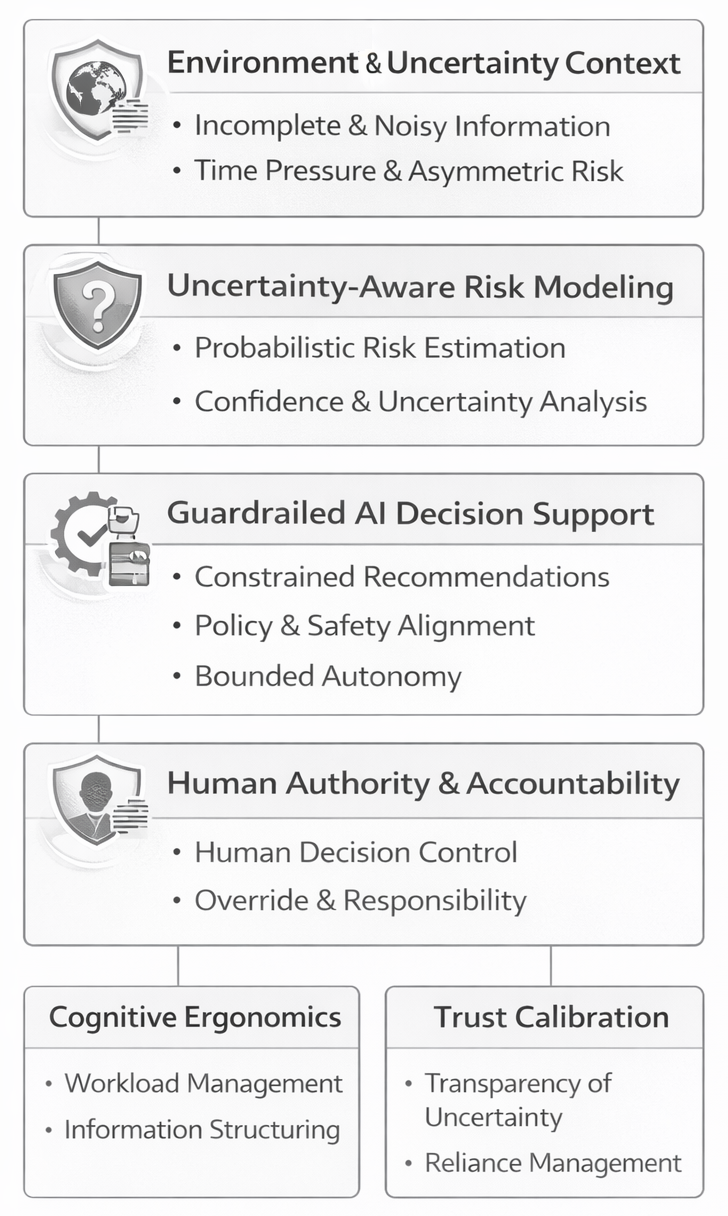
\includegraphics[width=0.60\linewidth]{fig_achdf_concept.png}
%DIFDELCMD <         \caption{Conceptual design layers of the Action-Centered Human--AI Decision Framework (ACHDF).
%DIFDELCMD < The framework structures human--AI decision support into four layered components: environment and uncertainty context, uncertainty-aware risk modeling, guardrailed AI decision support, and preserved human authority and accountability. Trust calibration and cognitive ergonomics operate as cross-cutting design considerations that influence interaction quality and reliable action execution under uncertainty.}
%DIFDELCMD <         \label{fig:achdf_concept}
%DIFDELCMD <     \end{figure}
%DIFDELCMD < 

%DIFDELCMD <     \begin{figure}[t]
%DIFDELCMD <         \centering
%DIFDELCMD <         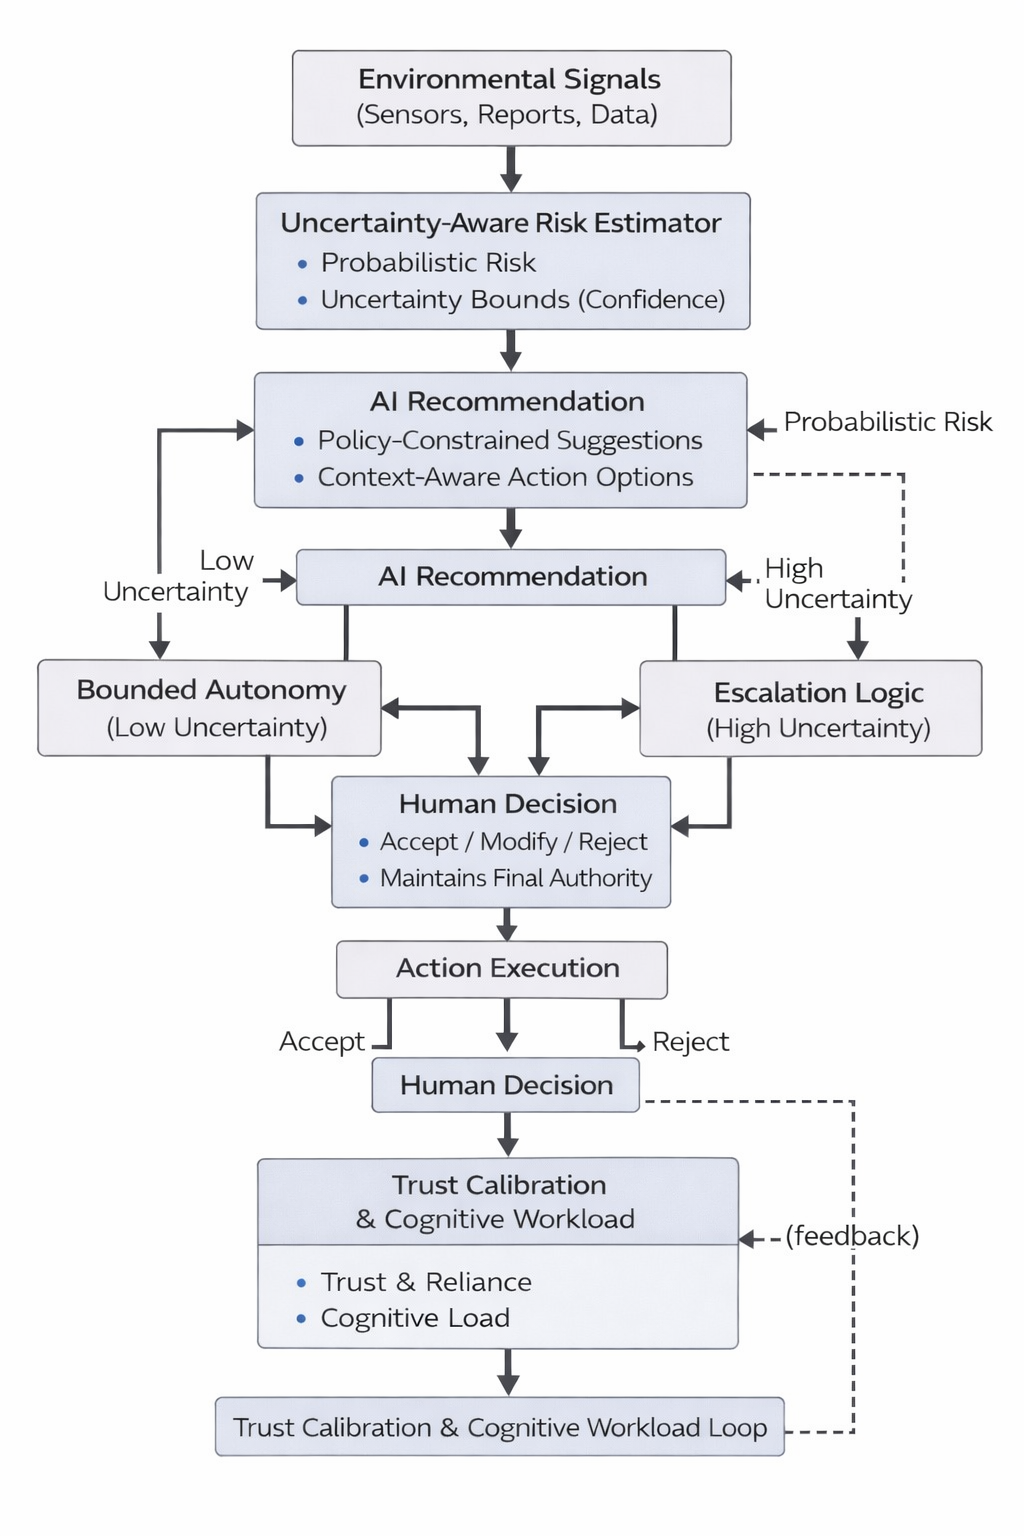
\includegraphics[width=0.95\linewidth]{fig_system_overview.png}
%DIFDELCMD <         \caption{Operational workflow of the proposed human--AI decision system.
%DIFDELCMD < Uncertainty-aware function allocation dynamically shifts decision authority between bounded autonomy and human-in-the-loop escalation.}
%DIFDELCMD <         \label{fig:system_overview}
%DIFDELCMD <     \end{figure}
%DIFDELCMD < %%%
\DIFdelend \DIFaddbegin \begin{figure}[t]
        \centering
        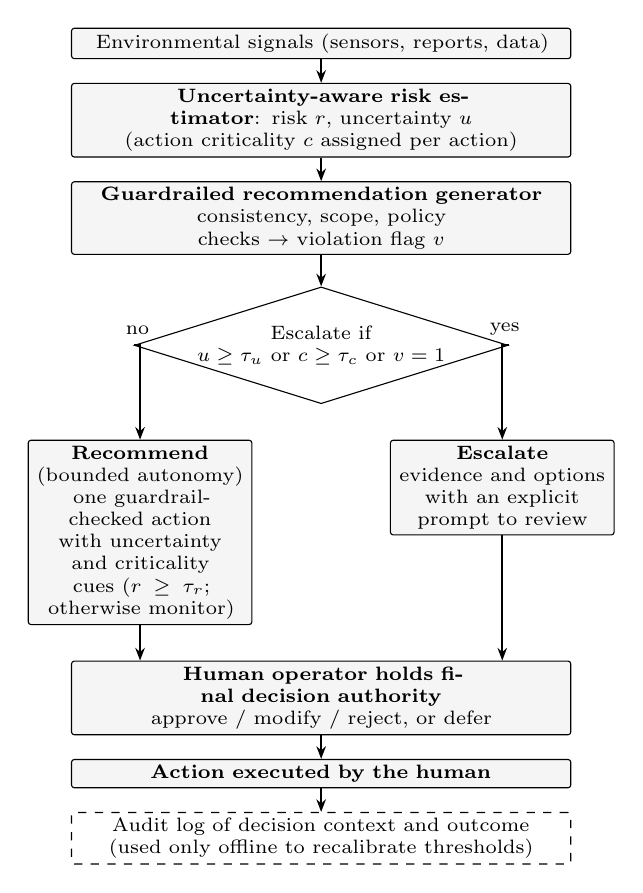
\begin{tikzpicture}[
            font=\scriptsize, node distance=3mm,
            box/.style={draw, rounded corners=1pt, align=center, fill=gray!8, text width=#1, inner sep=2pt},
            box/.default=6.2cm,
            dec/.style={draw, diamond, aspect=3.2, align=center, fill=white, inner sep=0pt},
            arr/.style={-{Stealth[length=1.6mm]}, thick}]
            \node[box] (env) {Environmental signals (sensors, reports, data)};
            \node[box, below=of env] (risk) {\textbf{Uncertainty-aware risk estimator}: risk $r$, uncertainty $u$\\(action criticality $c$ assigned per action)};
            \node[box, below=of risk] (gen) {\textbf{Guardrailed recommendation generator}\\consistency, scope, policy checks $\rightarrow$ violation flag $v$};
            \node[dec, below=4mm of gen] (pol) {Escalate if\\$u \ge \tau_u$ or $c \ge \tau_c$ or $v = 1$};
            \node[box=2.7cm, anchor=north] (rec) at ($(pol.south)+(-2.3,-0.45)$) {\textbf{Recommend} (bounded autonomy)\\one guardrail-checked action with uncertainty and criticality cues ($r \ge \tau_r$; otherwise monitor)};
            \node[box=2.7cm, anchor=north] (esc) at ($(pol.south)+(2.3,-0.45)$) {\textbf{Escalate}\\evidence and options with an explicit prompt to review};
            \node[box, anchor=north] (hum) at ($(rec.south -| pol.south)+(0,-0.45)$) {\textbf{Human operator holds final decision authority}\\approve / modify / reject, or defer};
            \node[box, below=of hum] (act) {\textbf{Action executed by the human}};
            \node[box, below=of act, fill=white, dashed] (log) {Audit log of decision context and outcome\\(used only offline to recalibrate thresholds)};
            \draw[arr] (env) -- (risk); \draw[arr] (risk) -- (gen); \draw[arr] (gen) -- (pol);
            \draw[arr] (pol.west) -| node[above, pos=0.3] {no} (rec.north);
            \draw[arr] (pol.east) -| node[above, pos=0.3] {yes} (esc.north);
            \draw[arr] (rec.south) -- (rec.south |- hum.north);
            \draw[arr] (esc.south) -- (esc.south |- hum.north);
            \draw[arr] (hum) -- (act); \draw[arr] (act) -- (log);
        \end{tikzpicture}
        \caption{Operational workflow of the proposed human--AI decision system.
The escalation test follows Algorithm~\ref{alg:escalation}. Depending on the estimated uncertainty, the action criticality, and the guardrail policy checks, the system either presents a bounded recommendation or escalates the case for human review with evidence and options (when $r < \tau_r$ and no trigger fires, the system only monitors). In both modes, the human operator holds final decision and execution authority. Trust and workload are not adapted at run time. The audit log is used only offline.}
        \label{fig:system_overview}
    \end{figure}
\DIFaddend 

    \section{System Overview and Architecture}
    \DIFdelbegin \DIFdel{This section is intended to introduce the proposed human--AI decision system. In addition, it is intended to introduce the architectural elements of }\DIFdelend \DIFaddbegin \label{sec:system}
    \DIFadd{This section introduces }\DIFaddend the proposed human--AI decision system. The \DIFdelbegin \DIFdel{proposed human--AI decision system is intended to be }\DIFdelend \DIFaddbegin \DIFadd{system is }\DIFaddend non-autonomous and human-centric\DIFdelbegin \DIFdel{. It is intended to have a balanced approach to human and algorithmic decision-making. The architectural elements of the proposed human--AI decision system are based on }\DIFdelend \DIFaddbegin \DIFadd{: the AI analyzes information and proposes options, and the human decides and acts. The architecture follows }\DIFaddend the \textbf{Action-Centered Human--AI Decision Framework (ACHDF)}\DIFdelbegin \DIFdel{. In the proposed framework, there is a significant emphasis on human action execution as the primary goal of the system.
}%DIFDELCMD < 

%DIFDELCMD <     %%%
\DIFdel{A conceptual overview of the proposed action-centered architecture is illustrated in Fig.~\ref{fig:achdf_concept}.
As shown in the figure, ACHDF is organized into four primary design layers. The }\DIFdelend \DIFaddbegin \DIFadd{, which, following the joint cognitive systems perspective \cite{Hollnagel2005JCS,Woods2006JCS}, treats the human operator and the AI as one decision system whose goal is appropriate human action.
}

    \DIFadd{ACHDF has four design layers: the }\DIFaddend \emph{environment and uncertainty context} \DIFdelbegin \DIFdel{layer captures }\DIFdelend \DIFaddbegin \DIFadd{(}\DIFaddend incomplete, time-pressured, \DIFdelbegin \DIFdel{and asymmetric risk conditionsthat characterize high-stakes decision ecologies. Built on top of this, the }\DIFdelend \DIFaddbegin \DIFadd{asymmetric-risk conditions), }\DIFaddend \emph{uncertainty-aware risk modeling} \DIFdelbegin \DIFdel{layer produces }\DIFdelend \DIFaddbegin \DIFadd{(}\DIFaddend probabilistic risk estimates \DIFdelbegin \DIFdel{together with explicit confidence and uncertaintybounds. These estimates are then translated into }\DIFdelend \DIFaddbegin \DIFadd{with explicit uncertainty), \emph{guardrailed AI decision support} (}\DIFaddend constrained, policy-aligned options\DIFdelbegin \DIFdel{within the \emph{guardrailed AI decision support} layer, which ensures that generated recommendations remain consistent with operational and safety constraints. Finally, the }\DIFdelend \DIFaddbegin \DIFadd{), and }\DIFaddend \emph{human authority and accountability} \DIFdelbegin \DIFdel{layer preserves human control through }\DIFdelend \DIFaddbegin \DIFadd{(}\DIFaddend oversight, override, and responsibility\DIFdelbegin \DIFdel{mechanisms. The two }\DIFdelend \DIFaddbegin \DIFadd{). Two }\DIFaddend cross-cutting elements\DIFdelbegin \DIFdel{shown at the bottom of the figure—trust calibration }\DIFdelend \DIFaddbegin \DIFadd{, appropriate trust \cite{Lee2004} }\DIFaddend and cognitive ergonomics\DIFdelbegin \DIFdel{—continuously shape how information is presented so that operators can act reliably under uncertainty}\DIFdelend \DIFaddbegin \DIFadd{, are design considerations (Table~\ref{tab:constructs}): they determined which cues are shown (e.g., explicit uncertainty indicators) and how much information is shown at once, but the implemented system neither measures nor adapts to them at run time}\DIFaddend .

    \DIFdelbegin \DIFdel{The dynamic operationalization of these layers in real-time decision making is depicted in }\DIFdelend Fig.~\ref{fig:system_overview} \DIFdelbegin \DIFdel{. 
This workflow view emphasizes how uncertainty-aware function allocation governs the interaction loop between AI and the human operator}\DIFdelend \DIFaddbegin \DIFadd{depicts the run-time behavior}\DIFaddend . When model \DIFdelbegin \DIFdel{confidence is high and risk is bounded}\DIFdelend \DIFaddbegin \DIFadd{uncertainty is low and the action is not critical}\DIFaddend , the system \DIFdelbegin \DIFdel{can provide }\DIFdelend \DIFaddbegin \DIFadd{presents a }\DIFaddend tightly scoped, action-oriented \DIFdelbegin \DIFdel{recommendations under bounded autonomy. As uncertainty or potential impact increases, the escalation logic routes decisions to a human-in-the-loop review process, where the operator can approve, modify, or reject the suggested action. The feedback paths shown in the figure highlight how action outcomes and operator responses contribute to ongoing trust calibration and workload management, forming a closed human--AI decision loop oriented toward reliable action execution rather than mere prediction display}\DIFdelend \DIFaddbegin \DIFadd{recommendation. We call this mode \emph{bounded autonomy}: the term refers only to the AI's freedom in \emph{generating} a recommendation, which is bounded by guardrails, and does not mean that the AI executes actions or holds decision authority. When uncertainty, criticality, or a policy check exceeds its threshold, the system switches to \emph{escalation}: instead of a single recommendation it presents the evidence and available options and explicitly asks the operator to review them. What varies between the two modes is thus the \emph{level and form of AI support}; final decision and execution authority stays with the human in both}\DIFaddend .

    \subsection{\DIFdelbegin \DIFdel{Design Goals }\DIFdelend \DIFaddbegin \DIFadd{Constructs }\DIFaddend and \DIFdelbegin \DIFdel{Human-in-the-Loop Principles}\DIFdelend \DIFaddbegin \DIFadd{Their Roles}\DIFaddend }
    \DIFdelbegin \DIFdel{The design of the proposed systemis informed by three key goals that are derived from the fundamental principles of ACHDF. }\DIFdelend \DIFaddbegin \label{sec:constructs}
    \DIFadd{Table~\ref{tab:constructs} summarizes the role of each ACHDF construct, i.e., whether it is a design input, a system state, a design consideration, or an evaluation outcome, together with its operational definition in the implemented system.
}\DIFaddend 

\DIFaddbegin \begin{table*}[t]
\centering
\caption{ACHDF Constructs: Role, Operational Definition, and Implementation}
\label{tab:constructs}
\begin{tabular}{p{2.4cm} p{3.4cm} p{10.6cm}}
\toprule
\textbf{Construct} & \textbf{Role in ACHDF} & \textbf{Operational definition / implementation} \\
\midrule
Uncertainty $u$ & Design input; determines system mode & Dispersion of the posterior risk estimate (Section~\ref{sec:risk}); compared with threshold $\tau_u$. \\
Criticality $c$ & Design input; determines system mode & Severity of the consequences if the recommended action is wrong or delayed (cost of error); compared with threshold $\tau_c$. \\
Guardrails & Constraint on recommendation generation & Rule-based checks on every recommendation (Section~\ref{sec:guardrails}). In the framework, a failed check withholds the recommendation and escalates the case ($v=1$ in Algorithm~\ref{alg:escalation}); in the study prototype, a deny-list hit redacts the text instead. \\
Bounded autonomy & System mode (``recommend'') & The AI presents one scoped, guardrail-checked recommendation. The AI never executes actions; the human decides and acts. \\
Escalation & System mode (``escalate'') & Triggered if $u \ge \tau_u$, $c \ge \tau_c$, or a policy check fails ($v=1$). The system presents evidence and options and asks the operator to approve, modify, or reject. \\
Trust & Design consideration; secondary outcome & Shaped interface design (explicit uncertainty and criticality cues). Measured post-condition by questionnaire (Section~\ref{sec:measures}). Not adapted at run time. \\
Workload & Design consideration; secondary outcome & Shaped interface design (single consolidated view, action-oriented phrasing). Measured post-condition by NASA--TLX \cite{Hart1988}. Not adapted at run time. \\
Action execution & Primary outcome & Measured by AER (Section~\ref{sec:measures}). \\
\bottomrule
\end{tabular}
\end{table*}

    \subsection{\DIFadd{Design Goals}}
    \DIFadd{Three goals follow from ACHDF. }\DIFaddend \textbf{Goal 1\DIFdelbegin \DIFdel{— Enabling Human Action Execution.}\DIFdelend \DIFaddbegin \DIFadd{:}\DIFaddend } \DIFdelbegin \DIFdel{The proposed system must be able to support }\DIFdelend \DIFaddbegin \DIFadd{enable human }\DIFaddend \emph{\DIFdelbegin \DIFdel{human }\DIFdelend action execution\DIFdelbegin %DIFDELCMD < \MBLOCKRIGHTBRACE %%%
\DIFdel{effectively, as opposed to simply improving }\DIFdelend \DIFaddbegin }\DIFadd{, not only }\DIFaddend situational awareness and prediction accuracy. \DIFdelbegin \DIFdel{The key goal of the proposed system is therefore to enable effective human decision-making and action in operational settings.
}%DIFDELCMD < 

%DIFDELCMD <     %%%
\DIFdelend \textbf{Goal 2\DIFdelbegin \DIFdel{— Supporting Calibrated Trust.}\DIFdelend \DIFaddbegin \DIFadd{:}\DIFaddend } \DIFdelbegin \DIFdel{The proposed system must }\DIFdelend support appropriate trust \DIFdelbegin \DIFdel{calibration by making its uncertainty , model limitations, and potential failure modes explicit. By doing so, the proposed system enables users to develop a realistic understanding of when to trust the system 's outputs and when to trust human judgment. }%DIFDELCMD < 

%DIFDELCMD <     %%%
\DIFdelend \DIFaddbegin \DIFadd{\cite{Lee2004} by making uncertainty explicit, so that users can judge when to rely on the system and when on their own judgment. }\DIFaddend \textbf{Goal 3\DIFdelbegin \DIFdel{- Preserving Human Authority.}\DIFdelend \DIFaddbegin \DIFadd{:}\DIFaddend } \DIFdelbegin \DIFdel{The system shall ensure the preservation of human authorityin high-risk decisions by incorporating human-in-the-loop mechanisms and bounded autonomy. This means that, in safety-critical or ethically critical situations, the system will ensure that human operators have the }\DIFdelend \DIFaddbegin \DIFadd{preserve human authority: operators always hold }\DIFaddend final decision-making \DIFdelbegin \DIFdel{authority, avoiding over-reliance on automation or artificial intelligence. }%DIFDELCMD < 

%DIFDELCMD <     %%%
\DIFdel{To ensure that these goals are achieved, the system will employ a human--AI collaboration paradigm, where the AI will be used to provide decision scaffolding and action-oriented recommendations, and the human will have the final responsibility for executing actions. The system will employ automation that assists in information synthesis and option generation, but will not be used for executing irreversible actions. This ensures the implementationof the concept of uncertainty-governed function allocation, where the level of automation will be dynamically adapted according to the level of uncertainty and criticality of actions}\DIFdelend \DIFaddbegin \DIFadd{and execution authority. In the terms of Parasuraman \emph{et al.} \cite{Parasuraman2000LOA}, the system automates information analysis and decision selection but not action implementation, and the level and form of support adapt to the estimated uncertainty and the criticality of the action}\DIFaddend .

    \subsection{Probabilistic Risk Estimation With Uncertainty}
    \DIFdelbegin \DIFdel{The heart of the system is a probabilistic risk estimation module that provides calibrated risk assessments along with uncertainty representations. Unlike many models that produce point estimate results, the model provides posterior risk distributions that include data-driven variability and epistemic uncertainty}\DIFdelend \DIFaddbegin \label{sec:risk}
    \DIFadd{Rather than a point estimate, the risk module outputs a posterior risk distribution, from which the risk level $r$ and the uncertainty $u$ are derived; together they determine whether the system presents a bounded recommendation or escalates (Algorithm~\ref{alg:escalation}). Explicit uncertainty is intended to avoid conveying false precision. This paper focuses on how the estimate and its uncertainty are used in the human--AI interaction, not on the risk model itself, whose estimation and calibration are not evaluated here (Section~\ref{sec:lim_reporting})}\DIFaddend .

    \textbf{\DIFdelbegin \DIFdel{Role 1 in ACHDF}\DIFdelend \DIFaddbegin \DIFadd{Study prototype configuration}\DIFaddend .} \DIFdelbegin \DIFdel{These estimates of uncertainty are a crucial part of the decision logic}\DIFdelend \DIFaddbegin \DIFadd{The prototype used the configuration of the open reference implementation distributed with the paper (confirmed by the author): a Bayesian linear regression with a Gaussian prior on four normalized factors (hazard, exposure, vulnerability entered as $1-$vulnerability, and a social factor) plus an intercept (noise variance $\sigma^2=0.10$, prior variance $\tau^2=2.0$)}\DIFaddend . The risk level \DIFdelbegin \DIFdel{is interpreted in conjunction with the confidence intervals to determine whether the system should make recommendations on its own or whether the process should be deferred to humans. The system’s explicit representation of its own uncertainties helps to prevent the propagation of false precision and supports the reasoning of the risk level in a way that mirrors the human decision-making process}\DIFdelend \DIFaddbegin \DIFadd{$r$ is the posterior mean prediction clipped to $[0,1]$, and $u$ is the posterior variance. Two thresholds on $r$ yield an ``IMMEDIATE'' ($r \ge 0.8$), ``PREPARE'' ($0.6 \le r < 0.8$), or ``STAY ALERT'' ($r < 0.6$) message; a further configured value (0.3) is unused. These three levels are coarser than the five response options of the task (Section~\ref{sec:task}) and do not map one-to-one onto them. The configuration specifies no values for $\tau_u$ and $\tau_c$ and contains no code for the escalation branch of Algorithm~\ref{alg:escalation}: the algorithm is the framework specification, and in the study the escalation flag was pre-assigned per trial in the scenario design and logged}\DIFaddend .

    \subsection{Guardrailed AI Recommendation Module}
    \DIFdelbegin \DIFdel{To make risk estimates actionable and provide appropriate recommendations, a generative AI module is used by }\DIFdelend \DIFaddbegin \label{sec:guardrails}
    \DIFadd{The recommendation module converts the risk estimate into a recommended action with a short justification. In the prototype, the text comes from three fixed message templates selected by risk band, so the output is template-based, not free-form generation. In the framework, every recommendation passes three guardrail checks before it is shown: (i) a \emph{consistency check}, so that the action does not contradict the risk estimate; (ii) a \emph{scope check}, so that }\DIFaddend the \DIFdelbegin \DIFdel{system. }%DIFDELCMD < 

%DIFDELCMD <     %%%
\DIFdel{\textbf{Role 2 in ACHDF}
    The system is constrained by a number of layers of structural guardrails that provide assurance with regard to reliability, consistency, and compliance with policies. These guardrails ensure that the recommendations generated by the system align with the risk estimates that were made previously and that there is no contradiction with those estimates.
    There are also further constraints that restrict the scope of recommendations based on }\DIFdelend \DIFaddbegin \DIFadd{action comes from the set of permitted actions for the scenario; and (iii) a \emph{policy check}, for compliance with }\DIFaddend operational and safety \DIFdelbegin \DIFdel{considerations. These recommendations also provide context cues that indicate the criticality and confidence levels associated with them, thereby avoiding information processing and facilitating a smooth transition to decisions and actions under pressure.
By bounding the generative results within a structured decision process, the system harnesses the flexibility of generative AI while also limiting the risks of hallucination and overgeneralization, thereby ensuring that AI support is assistive rather than prescriptive. }%DIFDELCMD < \begin{algorithm}[t]
%DIFDELCMD <         \caption{Uncertainty-aware escalation and human override policy}
%DIFDELCMD <         \label{alg:escalation}
%DIFDELCMD <         \begin{algorithmic}[1]
%DIFDELCMD <             \Require risk estimate $r$, uncertainty $u$, action criticality $c$
%DIFDELCMD <             \Require thresholds $\tau_r, \tau_u, \tau_c$
%DIFDELCMD <             \State $\textsc{mode} \leftarrow \text{``assist''}$
%DIFDELCMD <             \If{$u \ge \tau_u$ \textbf{or} $c \ge \tau_c$}
%DIFDELCMD <             \State $\textsc{mode} \leftarrow \text{``escalate''}$ \Comment{route to human review}
%DIFDELCMD <             \ElsIf{$r \ge \tau_r$}
%DIFDELCMD <             \State $\textsc{mode} \leftarrow \text{``recommend''}$
%DIFDELCMD <             \Else
%DIFDELCMD <             \State $\textsc{mode} \leftarrow \text{``monitor''}$
%DIFDELCMD <             \EndIf
%DIFDELCMD <             \If{$\textsc{mode} = \text{``escalate''}$}
%DIFDELCMD <             \State Present evidence and options to operator
%DIFDELCMD <             \State Operator selects: approve / modify / reject
%DIFDELCMD <             \Else
%DIFDELCMD <             \State Generate bounded recommendation via guardrails
%DIFDELCMD <             \EndIf
%DIFDELCMD <             \State Log decision context and outcome for audit and calibration
%DIFDELCMD <         \end{algorithmic}
%DIFDELCMD <     \end{algorithm}
%DIFDELCMD <     %%%
\DIFdelend \DIFaddbegin \DIFadd{rules. A recommendation that fails any check is withheld and the case is escalated ($v=1$).
}\DIFaddend 

    \DIFdelbegin \subsection{\DIFdel{Human Override and Escalation Mechanisms}}
%DIFAUXCMD
\addtocounter{subsection}{-1}%DIFAUXCMD
\DIFdel{The escalation process, as described in Algorithm~\ref{alg:escalation}, is linked to an uncertainty-aware policy that is used to dynamically allocate authority depending on the level of uncertainty and the criticality of the actions taken. The human override and escalation mechanism is an important }\DIFdelend \DIFaddbegin \DIFadd{\textbf{Implementation in the study prototype.} Because the message is selected deterministically from $r$, it cannot contradict the risk estimate and is always a permitted message. The policy check is a deny-list filter (terms such as ``medical diagnosis'' and ``evacuation by force'' are replaced by ``}[\DIFadd{REDACTED}]\DIFadd{'', case-insensitively) plus expansion of technical terms into plain language. In the prototype, a policy hit therefore redacts text instead of triggering escalation; routing $v=1$ to escalation is }\DIFaddend part of the \DIFdelbegin \DIFdel{overall system architecture. The system automatically escalates decisions to human operators if the level of uncertainty is above certain thresholds, the potential impact of the recommendation is high, and if certain policy constraints are violated.
    In fact, escalation }\DIFdelend \DIFaddbegin \DIFadd{framework specification only. The criticality scale and its threshold $\tau_c$ are not documented. Each recommendation is displayed with criticality and confidence cues.
    }\begin{algorithm}[t]
        \caption{Uncertainty-aware escalation and human override policy}
        \label{alg:escalation}
        \begin{algorithmic}[1]
            \Require risk estimate $r$, uncertainty $u$, action criticality $c$
            \Require policy-violation flag $v \in \{0,1\}$ from guardrail checks
            \Require thresholds $\tau_r, \tau_u, \tau_c$
            \If{$u \ge \tau_u$ \textbf{or} $c \ge \tau_c$ \textbf{or} $v = 1$}
            \State $\textsc{mode} \leftarrow \text{``escalate''}$ \Comment{route to human review}
            \ElsIf{$r \ge \tau_r$}
            \State $\textsc{mode} \leftarrow \text{``recommend''}$ \Comment{bounded autonomy}
            \Else
            \State $\textsc{mode} \leftarrow \text{``monitor''}$
            \EndIf
            \If{$\textsc{mode} = \text{``escalate''}$}
            \State Present evidence and options to operator
            \State Operator selects: approve / modify / reject / defer
            \ElsIf{$\textsc{mode} = \text{``recommend''}$}
            \State Present guardrail-checked recommendation
            \State Operator decides and executes, overrides, or defers
            \EndIf
            \State Log decision context and outcome for audit and calibration
        \end{algorithmic}
    \end{algorithm}

\subsection{\DIFadd{Human Override and Escalation Mechanisms}}
\DIFadd{Escalation follows Algorithm~\ref{alg:escalation}: a case is escalated if uncertainty exceeds $\tau_u$, criticality exceeds $\tau_c$, or a guardrail check fails ($v=1$). Escalation }\DIFaddend is not a failure mode but a \DIFdelbegin \DIFdel{decision to escalate to ensure accountability under uncertain conditions. The operators are free to either }\DIFdelend \DIFaddbegin \DIFadd{deliberate change in the form of support that keeps the operator accountable. In every mode, operators can }\DIFaddend accept, modify, or reject the \DIFdelbegin \DIFdel{decision recommended by the AIsystem}\DIFdelend \DIFaddbegin \DIFadd{AI's recommendation}\DIFaddend , and all \DIFdelbegin \DIFdel{of these operations are recorded for accountability purposes. This minimization of processing of superfluous information is also beneficial for the management of cognitive workload for time-critical situations.
This dynamic allocation of autonomy allows the system to offer effective assistance in regular situations and }\DIFdelend \DIFaddbegin \DIFadd{operations are logged. This adaptation of the level of support follows established principles of adaptive automation \cite{Parasuraman2000LOA,Scerbo2007} and does not transfer decision authority to the AI.
}


    %DIF >  -------------------------------\input{./060-evaluation}
    \section{\DIFadd{Experimental Design and Methods}}

    \DIFadd{This section describes the controlled user study that compared the ACHDF-based system with a conventional dashboard; it is the only empirical evaluation reported. All statistics were recomputed from the anonymized trial-level logs (1}\DIFaddend ,\DIFdelbegin \DIFdel{at the same time, allow human control in uncertain or risky situations, thus striking a proper balance between performance and safety, as per the existing design principles for human--machine systems, which provides a platform for the ACHDF design principles proposed later in the paper.
}\DIFdelend \DIFaddbegin \DIFadd{040 trials) and questionnaire records, and the data and analysis scripts are provided with the paper (Section~\ref{sec:data}). Details that remain undocumented are listed in Section~\ref{sec:lim_reporting}.
}\DIFaddend 

    \DIFdelbegin %DIFDELCMD < \begin{table*}[t]
%DIFDELCMD < \centering
%DIFDELCMD < \caption{Transferability of ACHDF Design Principles Across Decision Ecologies}
%DIFDELCMD < \label{tab:achdf_transferability}
%DIFDELCMD < \begin{tabular}{p{3cm} p{3.2cm} p{3.2cm} p{2.8cm} p{3.9cm}}
%DIFDELCMD < \hline
%DIFDELCMD < \textbf{Decision Domain} &
%DIFDELCMD < \textbf{Primary Sources of Uncertainty} &
%DIFDELCMD < \textbf{Asymmetry of Error Costs} &
%DIFDELCMD < \textbf{Time Pressure Characteristics} &
%DIFDELCMD < \textbf{Role of Uncertainty-Aware Function Allocation} \\
%DIFDELCMD < \hline
%DIFDELCMD < Disaster Response &
%DIFDELCMD < Incomplete situational awareness, noisy sensor and report data, rapidly evolving conditions &
%DIFDELCMD < Delayed action leads to loss of life or property; false alarms incur operational cost &
%DIFDELCMD < Severe time pressure with dynamic escalation requirements &
%DIFDELCMD < AI provides bounded, action-oriented recommendations under low uncertainty; high uncertainty triggers human-in-the-loop escalation to preserve accountability \\
%DIFDELCMD < 

%DIFDELCMD < Autonomous Driving Supervision &
%DIFDELCMD < Perception uncertainty, rare edge cases, environment variability &
%DIFDELCMD < False negatives may cause accidents; false positives reduce efficiency and trust &
%DIFDELCMD < Sub-second to seconds-level response requirements &
%DIFDELCMD < Low-uncertainty situations allow bounded autonomy; ambiguous or novel situations escalate to human supervision and override \\
%DIFDELCMD < 

%DIFDELCMD < Medical AI (Triage / Diagnosis) &
%DIFDELCMD < Incomplete patient data, population-to-individual generalization limits &
%DIFDELCMD < False negatives risk patient harm; false positives cause overtreatment &
%DIFDELCMD < Moderate to high time pressure depending on clinical context &
%DIFDELCMD < AI assists with risk stratification and option generation; high uncertainty or high criticality decisions defer to clinicians \\
%DIFDELCMD < 

%DIFDELCMD < Military Safety Automation &
%DIFDELCMD < Adversarial uncertainty, incomplete intelligence, strategic deception &
%DIFDELCMD < Incorrect action may cause catastrophic or irreversible consequences &
%DIFDELCMD < High time pressure combined with strategic deliberation &
%DIFDELCMD < AI supports sensemaking and constrained recommendations; final decision authority remains with human operators under uncertainty \\
%DIFDELCMD < 

%DIFDELCMD < \hline
%DIFDELCMD < \end{tabular}
%DIFDELCMD < \end{table*}
%DIFDELCMD < %%%
\DIFdelend \DIFaddbegin \subsection{\DIFadd{Study Design and Conditions}}
\DIFaddend 

    \DIFdelbegin \subsection{\DIFdel{ACHDF Transferability Across Decision Ecologies}}
%DIFAUXCMD
\addtocounter{subsection}{-1}%DIFAUXCMD
\DIFdel{Although the system architecture is instantiated and verified in the context of disaster response, the design principles are not domain-specific in nature.On the contrary, the architecture presented here is more aligned with a general class of \emph{decision ecologies} that are characterized by high uncertainty, asymmetrical costs of errors, timing pressures, and human accountability. }\DIFdelend \DIFaddbegin \DIFadd{We used a within-subjects design with a \emph{baseline} and an \emph{AI-assisted} (ACHDF) condition in counterbalanced order (28 participants completed the AI-assisted condition first, 24 the baseline first). Both conditions were designed to present comparable scenario sets. Counterbalancing does not remove carry-over, since participants may have remembered scenarios from the first condition, so we tested order and carry-over effects (Section~\ref{sec:res_order}).
}

    \DIFadd{\textbf{Baseline condition.} Participants used a conventional dashboard-style interface (Fig.~\ref{fig:interfaces}a): a risk-level summary (numeric value and color coding), a map or time series of risk indicators, and the five response-option buttons. It provided no AI-generated recommendation, uncertainty indicator, criticality cue, or escalation prompt, so participants had to integrate the information themselves.
}

    \DIFadd{\textbf{AI-assisted condition.} }\DIFaddend The \DIFdelbegin \DIFdel{\textbf{Action-Centered Human--AI Decision Framework (ACHDF)} is intended to be more general in nature to cover a range of different safety-critical domains that have similar structural characteristics}\DIFdelend \DIFaddbegin \DIFadd{ACHDF-based interface displayed the same underlying information plus the ACHDF features of Section~\ref{sec:system}: a risk estimate with an uncertainty indicator (a confidence interval or variance proxy), a criticality badge, and either a single guardrail-checked recommendation with a short rationale (``recommend'' mode, e.g., ``PREPARE: Pack essentials, confirm route to shelter, check on neighbors.'') or, when escalation was triggered, the evidence and options with a message that human review was required because of uncertainty, criticality, or a policy issue (``escalate'' mode). The five response options remained selectable in both modes, so participants could ignore the recommendation, and both interfaces supported a deferral flag. Table~\ref{tab:conditions} and Fig.~\ref{fig:interfaces} contrast the two interfaces; the decision logic is in Fig.~\ref{fig:system_overview} and Algorithm~\ref{alg:escalation}. Fig.~\ref{fig:interfaces} is a reconstructed illustration drawn from the interface specification, not a screenshot; no screenshots of the study interface are available (Section~\ref{sec:lim_reporting})}\DIFaddend .

    \DIFdelbegin \DIFdel{In order to further illustrate the general nature of the design principles presented in this work, Table \ref{tab:achdf_transferability} provides a decision ecology mapping that illustrates the transferability of the design principles to different application domains that are presented in this paper, such as the supervision of autonomous driving, medical AI in the context of medical triage or diagnostic support systems, or military safety automation systems.
Despite the varying nature of the uncertainty in each of the application domains considered in this paper, }\DIFdelend \DIFaddbegin \begin{figure*}[t]
        \centering
        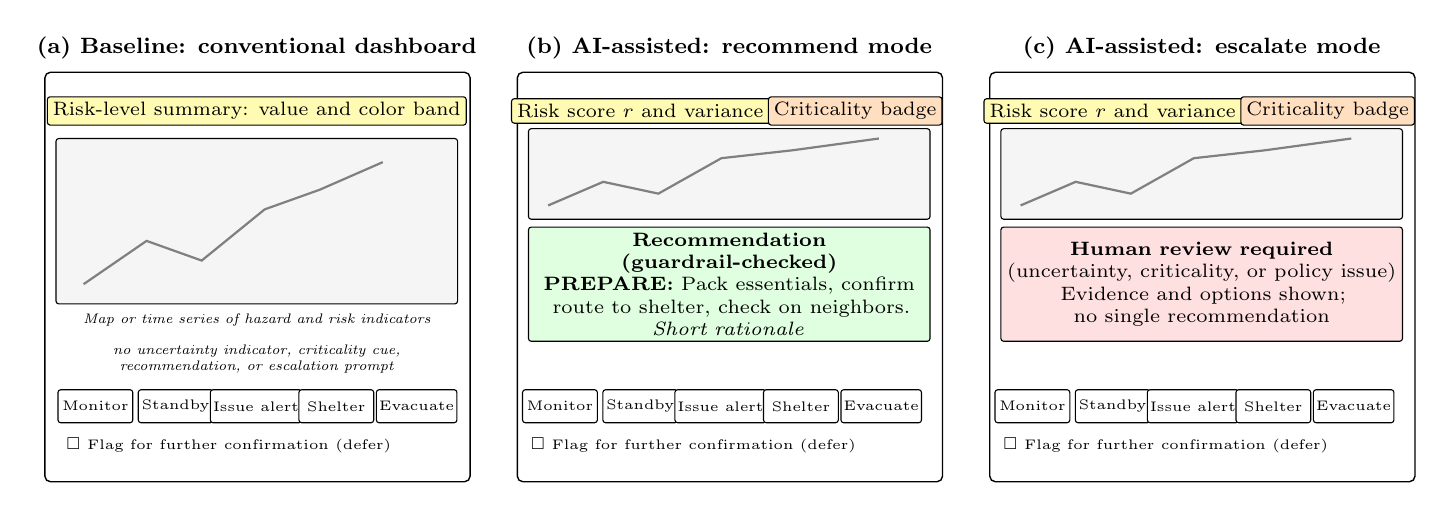
\begin{tikzpicture}[font=\scriptsize,
            frame/.style={draw, rounded corners=2pt, line width=0.5pt, fill=white},
            blk/.style={draw, rounded corners=1pt, align=center, inner sep=2pt, fill=gray!8},
            btn/.style={draw, rounded corners=1pt, align=center, inner sep=1pt, minimum height=0.42cm, fill=white, font=\tiny},
            ttl/.style={font=\footnotesize\bfseries}]
        % ---------- helper: five option buttons + defer flag, drawn at given x-offset and y
        \newcommand{\optionrow}[2]{%
          \node[btn, minimum width=0.95cm] at (#1+0.55,#2) {Monitor};
          \node[btn, minimum width=0.95cm] at (#1+1.57,#2) {Standby};
          \node[btn, minimum width=0.95cm] at (#1+2.59,#2) {Issue alert};
          \node[btn, minimum width=0.95cm] at (#1+3.61,#2) {Shelter};
          \node[btn, minimum width=0.95cm] at (#1+4.63,#2) {Evacuate};
          \node[anchor=west, font=\tiny] at (#1+0.05,#2-0.5) {$\square$ Flag for further confirmation (defer)};}
        % ---------- (a) baseline
        \node[ttl] at (2.6,0.45) {(a) Baseline: conventional dashboard};
        \node[frame, minimum width=5.4cm, minimum height=5.2cm, anchor=north west] (fa) at (-0.1,0.15) {};
        \node[blk, fill=yellow!30, minimum width=5.1cm] at (2.6,-0.35) {Risk-level summary: value and color band};
        \node[blk, minimum width=5.1cm, minimum height=2.1cm] at (2.6,-1.75) {};
        \draw[gray, thick] (0.4,-2.55) -- (1.2,-2.0) -- (1.9,-2.25) -- (2.7,-1.6) -- (3.4,-1.35) -- (4.2,-1.0);
        \node[font=\tiny\itshape] at (2.6,-3.0) {Map or time series of hazard and risk indicators};
        \node[font=\tiny\itshape, align=center] at (2.6,-3.5) {no uncertainty indicator, criticality cue,\\recommendation, or escalation prompt};
        \optionrow{-0.0}{-4.1}
        % ---------- (b) AI recommend
        \node[ttl] at (8.6,0.45) {(b) AI-assisted: recommend mode};
        \node[frame, minimum width=5.4cm, minimum height=5.2cm, anchor=north west] at (5.9,0.15) {};
        \node[blk, fill=yellow!30, minimum width=3.2cm] at (7.6,-0.35) {Risk score $r$ and variance $u$};
        \node[blk, fill=orange!25, minimum width=1.7cm] at (10.2,-0.35) {Criticality badge};
        \node[blk, minimum width=5.1cm, minimum height=1.15cm] at (8.6,-1.15) {};
        \draw[gray, thick] (6.3,-1.55) -- (7.0,-1.25) -- (7.7,-1.4) -- (8.5,-0.95) -- (9.4,-0.85) -- (10.5,-0.7);
        \node[blk, fill=green!12, minimum width=5.1cm, text width=4.9cm, minimum height=1.45cm] at (8.6,-2.55) {\textbf{Recommendation (guardrail-checked)}\\ \textbf{PREPARE:} Pack essentials, confirm route to shelter, check on neighbors.\\ \emph{Short rationale}};
        \optionrow{5.9}{-4.1}
        % ---------- (c) AI escalate
        \node[ttl] at (14.6,0.45) {(c) AI-assisted: escalate mode};
        \node[frame, minimum width=5.4cm, minimum height=5.2cm, anchor=north west] at (11.9,0.15) {};
        \node[blk, fill=yellow!30, minimum width=3.2cm] at (13.6,-0.35) {Risk score $r$ and variance $u$};
        \node[blk, fill=orange!25, minimum width=1.7cm] at (16.2,-0.35) {Criticality badge};
        \node[blk, minimum width=5.1cm, minimum height=1.15cm] at (14.6,-1.15) {};
        \draw[gray, thick] (12.3,-1.55) -- (13.0,-1.25) -- (13.7,-1.4) -- (14.5,-0.95) -- (15.4,-0.85) -- (16.5,-0.7);
        \node[blk, fill=red!12, minimum width=5.1cm, text width=4.9cm, minimum height=1.45cm] at (14.6,-2.55) {\textbf{Human review required}\\ (uncertainty, criticality, or policy issue)\\ Evidence and options shown; no single recommendation};
        \optionrow{11.9}{-4.1}
        \end{tikzpicture}
        \caption{Reconstructed illustration of the two study interfaces, drawn from the interface specification. It is \emph{not} a screenshot: layout and colors are approximate and the values are placeholders; the recommendation wording follows the prototype's template. In the AI-assisted condition, panel (b) or (c) is shown for a given trial. In both conditions, the human selects the final action from the same five options and can flag a deferral.}
        \label{fig:interfaces}
    \end{figure*}

    \begin{table}[t]
        \caption{Information and Features Presented in Each Condition}
        \label{tab:conditions}
        \centering
        \begin{tabular}{p{0.40\linewidth}cc}
            \toprule
            \textbf{Element} & \textbf{Baseline} & \textbf{AI-assisted} \\
            \midrule
            Hazard and risk information & \cmark & \cmark \\
            Explicit uncertainty indicator & \xmark & \cmark \\
            Criticality cue & \xmark & \cmark \\
            Guardrail-checked action recommendation & \xmark & \cmark$^{a}$ \\
            Escalation prompt with evidence and options & \xmark & \cmark$^{b}$ \\
            Human decides and executes & \cmark & \cmark \\
            \bottomrule
            \multicolumn{3}{p{0.93\linewidth}}{\footnotesize $^{a}$ In ``recommend'' mode. $^{b}$ In ``escalate'' mode, which replaced the single recommendation in 150 of the 520 AI-assisted trials (28.8\%).}
        \end{tabular}
    \end{table}

    \DIFadd{Because the AI-assisted condition differs from the baseline in several features at once (recommendation, action-oriented format, uncertainty cue, criticality cue, and escalation), }\DIFaddend the \DIFdelbegin \DIFdel{role of uncertainty-aware function allocation is similar in nature. The contribution of this work is not about optimizing any particular domain or application scenario in the context of human--AI decisions under uncertainty.
}\DIFdelend \DIFaddbegin \DIFadd{comparison estimates the effect of the integrated ACHDF configuration, not of any single feature.
}\DIFaddend 

    %DIF <  -------------------------------\input{./060-evaluation}
    \DIFdelbegin \section{\DIFdel{Experimental Design and Methods}}
%DIFAUXCMD
\addtocounter{section}{-1}%DIFAUXCMD
\DIFdelend \DIFaddbegin \subsection{\DIFadd{Participants and Ethics}}
    \label{sec:participants}
\DIFaddend 

    \DIFdelbegin \DIFdel{In this section, we describe the design of the experiments that can be used to test the proposed human--AI decision system. In our case, we aimed to isolate the effect of AI support on human action execution, response behavior, and subjective experience. In general, our design of experiments follows the usual practice of designing experiments to evaluate human--machine systems, where experiments are defined with clear conditions for baseline and treatment cases}\DIFdelend \DIFaddbegin \DIFadd{Fifty-two participants took part (age 37.2 $\pm$ 9.3 years, range 23--54; 28 male, 23 female, 1 other; technical background low/medium/high 19/16/17), recruited by stratified sampling for diversity in age, gender, and technical background. No prior domain expertise was required; none reported high prior disaster-response experience (23 none, 21 low, 8 medium), so the sample was not composed of trained emergency-management professionals (Section~\ref{sec:limitations}).
}

    \DIFadd{\textbf{Ethics.} Participation was voluntary, and all participants gave informed consent and consent to the processing of their personal information before the experiment. The study consisted of a simulated decision task, questionnaires, and short interviews, with no physical or medical intervention. Only age, gender, and technical and disaster-experience background were recorded; identifying information was removed from the survey spreadsheets before analysis, and the task logs contain no identifying information. The study was not submitted to an institutional review board (IRB): before the study, the author asked the author's institutional IRB and was advised that a survey-type study with no intervention on the human body is not subject to review, and that the IRB does not accept applications for such studies. The study involved no experiment on, contact with, or intervention in the human body, and no human-derived materials, drugs, or medical devices. No approval or exemption number exists for it. We regard the risk to participants as minimal, but this is the author's assessment, not a determination by an ethics body.
}

    \DIFadd{\textbf{Sample size.} No a priori power analysis was conducted; $n=52$ was not derived from an expected effect size. A sensitivity analysis shows that a two-sided paired $t$-test at $\alpha=.05$ has 80\% power to detect $d_z \geq 0.40$. The observed effects on the primary outcome ($d_z = 0.96$) and the secondary outcomes (smallest $|d_z| = 0.91$) are well above this value; smaller effects, such as some subscale differences, may not have been detected reliably}\DIFaddend .


    \subsection{\DIFdelbegin \DIFdel{Study Design }\DIFdelend \DIFaddbegin \DIFadd{Decision Task }\DIFaddend and \DIFdelbegin \DIFdel{Conditions (Baseline vs.\ AI-Assisted)}\DIFdelend \DIFaddbegin \DIFadd{Procedure}\DIFaddend }
    \DIFaddbegin \label{sec:task}
\DIFaddend 

    \DIFdelbegin \DIFdel{A within-subjects design was employed in the experiment. In this design, the participants are presented with the same decision-making task in two different conditions: a \emph{baseline} condition and an }\DIFdelend \DIFaddbegin \DIFadd{Each participant completed 10 decision trials in each condition (20 trials; 1,040 in total), labeled S01--S10 in the logs. In each trial, participants interpreted risk information about an evolving flood or flash-flood hazard in a synthetic region and selected one of five response options: }\DIFaddend \emph{\DIFdelbegin \DIFdel{AI-assisted}\DIFdelend \DIFaddbegin \DIFadd{monitor}\DIFaddend } \DIFdelbegin \DIFdel{condition. In the baseline condition, the participants were presented with the conventional dashboard-based interface. }\DIFdelend \DIFaddbegin \DIFadd{(continue observing; risk is low), \emph{standby} (prepare; risk is rising but it is not yet time to act), \emph{issue alert} (draw residents' attention to the situation), \emph{shelter in place} (stay indoors; moving is difficult or dangerous), or \emph{recommend evacuation} (risk is high; leaving is required). The reference (correct) action of each trial is recorded in the log. A trial presented the region, four risk factors (hazard, exposure, vulnerability, social), a risk score with its uncertainty, subgroup information (e.g., elderly, migrant), and a short situation description. Example descriptions in the study materials are a low-risk case (risk about 0.2; ``rainfall is increasing, but the risk of flooding in low-lying areas is still low; further observation is needed'', intended action: monitor) and a high-risk case (0.8 or more; ``the risk of a flash flood is imminent; immediate evacuation or sheltering is required'', intended action: shelter or evacuate). }\DIFaddend In the \DIFaddbegin \DIFadd{logs, however, the reference action stored for a scenario label does not follow this pattern (Section~\ref{sec:lim_reporting}), so these examples illustrate the design and cannot be matched to logged trials. Whether a trial was escalated was fixed in advance in the scenario design (some scenarios had high uncertainty or criticality and were shown in escalate mode), not computed at run time from $\tau_u$ and $\tau_c$. A logged }\DIFaddend AI-assisted \DIFdelbegin \DIFdel{condition, the participants were presented with the proposed system that provides context-aware recommendations through the human--AI decision architecture.To avoid learning effects and order effects in the experiment, the presentation order of }\DIFdelend \DIFaddbegin \DIFadd{record reads: participant P01, scenario S03, selected action \emph{monitor}, reference action \emph{monitor}, latency 7.9~s, escalation flagged, deferral flagged. Per-trial stimulus values (risk score, uncertainty, criticality) are not part of the records (Section~\ref{sec:lim_reporting}), and the longest recorded latency was 20.3~s. Participants could flag a trial as deferred pending further confirmation (the log records the flag together with the action finally selected); in }\DIFaddend the \DIFdelbegin \DIFdel{two conditions is counterbalanced. The significance of the results is determined by conducting a paired test. In both the baseline and }\DIFdelend AI-assisted \DIFdelbegin \DIFdel{conditions, the same data is used. Hence, the difference in the performance between the two conditions is solely due to the presence of AI assistance.
}%DIFDELCMD < 

%DIFDELCMD <     %%%
\subsection{\DIFdel{Participants and Sampling Strategy}}
%DIFAUXCMD
\addtocounter{subsection}{-1}%DIFAUXCMD
%DIFDELCMD < 

%DIFDELCMD <     %%%
\DIFdel{The demographics of participants are presented in Table~\ref{tab:participants}}\DIFdelend \DIFaddbegin \DIFadd{condition, escalation explicitly prompted such a review (Section~\ref{sec:res_escalation})}\DIFaddend .

    \DIFdelbegin %DIFDELCMD < \begin{table}[t]
%DIFDELCMD < 

%DIFDELCMD <         \caption{Participant Demographics}
%DIFDELCMD < 

%DIFDELCMD <         \label{tab:participants}
%DIFDELCMD < 

%DIFDELCMD <         \centering
%DIFDELCMD < 

%DIFDELCMD <         \begin{tabular}{l c}
%DIFDELCMD < 

%DIFDELCMD <             \hline
%DIFDELCMD < 

%DIFDELCMD <             Characteristic & Value \\
%DIFDELCMD < 

%DIFDELCMD <             \hline
%DIFDELCMD < 

%DIFDELCMD <             Total participants & 52 \\
%DIFDELCMD < 

%DIFDELCMD <             Age range & 20--50s \\
%DIFDELCMD < 

%DIFDELCMD <             Gender & Mixed \\
%DIFDELCMD < 

%DIFDELCMD <             Technical background & Low--High \\
%DIFDELCMD < 

%DIFDELCMD <             Study design & Within-subjects \\
%DIFDELCMD < 

%DIFDELCMD <             \hline
%DIFDELCMD < 

%DIFDELCMD <         \end{tabular}
%DIFDELCMD < 

%DIFDELCMD <     \end{table}
%DIFDELCMD < 

%DIFDELCMD <     %%%
\DIFdel{The total number of participants recruited for the study was 52 in number. For }\DIFdelend \DIFaddbegin \DIFadd{Before the trials, all participants received a training session covering (1) }\DIFaddend the purpose of \DIFdelbegin \DIFdel{this study, participants were recruited using the stratified sampling technique in order to create diversity in terms of age, gender, and technical know-how. This technique has been selected due to the heterogeneity observed in operators in real-world decision environments.
}%DIFDELCMD < 

%DIFDELCMD <     %%%
\DIFdel{All participants gave their informed consent prior to the experiment. Although participants were not required to have prior knowledge in the domain area, training on the task interface was provided to all participants to create uniformity in terms of familiarity with the procedures. }%DIFDELCMD < 

%DIFDELCMD <     %%%
\subsection{\DIFdel{Task Design and Procedure}}
%DIFAUXCMD
\addtocounter{subsection}{-1}%DIFAUXCMD
%DIFDELCMD < 

%DIFDELCMD <     %%%
\DIFdel{The participants were required to complete a set of time-sensitive decision tasks. These tasks involved understanding risk information and making a decision on whether or not to take a protective action. These decision tasks were aimed at capturing the essential aspects of a high-stakes decision situation. These aspects include changes in information, uncertainty, and unbalanced error costs.
}\DIFdelend \DIFaddbegin \DIFadd{the system and the human-in-the-loop principle (5~min), (2) the five response options and the asymmetric costs of errors (5~min), (3)--(4) a demonstration of each interface (for the AI-assisted one, recommend and escalate modes, the uncertainty indicator, the criticality cue, and the deferral flag), each followed by one practice trial, and (5) an introduction to the NASA--TLX, trust, and SUS questionnaires. Participants were told that the recommendation is only an aid that they could disregard and that the primary performance measure was the share of trials with the correct action; speed alone was not the criterion. }\DIFaddend The \DIFdelbegin \DIFdel{experiment involved a training period, and after that, the participants completed the task execution of both the experimental conditions. The participants were required to focus on the efficacy of the action rather than on the analysis of the information. The system was used to record the decision processes and interaction of the participants.
}%DIFDELCMD < 

%DIFDELCMD <     \begin{table}[t]
%DIFDELCMD <         \caption{Outcome measures used in the controlled study}
%DIFDELCMD <         \label{tab:measures}
%DIFDELCMD <         \centering
%DIFDELCMD <         \begin{tabular}{p{0.23\linewidth}p{0.70\linewidth}}
%DIFDELCMD <             \toprule
%DIFDELCMD <             \textbf{Measure} & \textbf{Operationalization} \\
%DIFDELCMD <             \midrule
%DIFDELCMD <             Response Latency & Time from presentation of actionable information to action execution. \\
%DIFDELCMD <             Cognitive Workload & NASA--TLX overall score and subscales (post-condition). \\
%DIFDELCMD <             Trust & Post-task Likert-type items on perceived reliability, predictability, and appropriateness of recommendations. \\
%DIFDELCMD <             Usability & Standard usability scale (post-condition). \\
%DIFDELCMD <             \bottomrule
%DIFDELCMD <         \end{tabular}
%DIFDELCMD <     \end{table}
%DIFDELCMD < 

%DIFDELCMD <     %%%
%DIF < ------------------------------------------------------
%DIFDELCMD < 

%DIFDELCMD <     \begin{figure}[t]
%DIFDELCMD <         \centering
%DIFDELCMD <         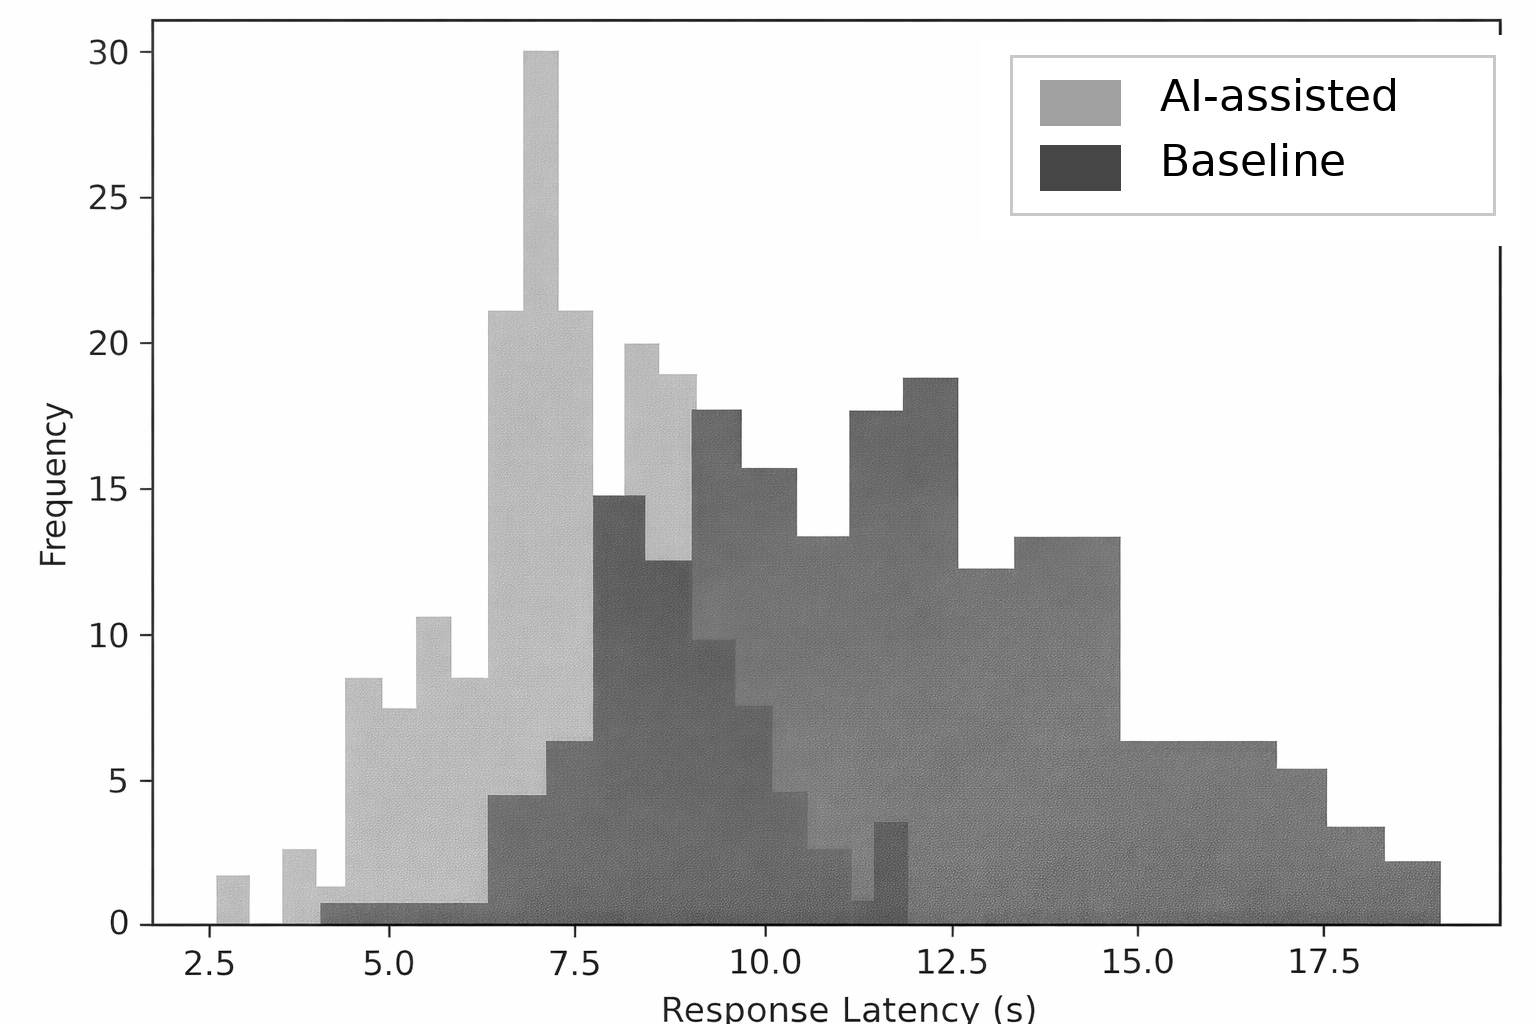
\includegraphics[width=0.9\linewidth]{fig_latency_distribution.png}
%DIFDELCMD <         \caption{Distribution of response latency under baseline and AI-assisted conditions. The distribution under the AI-assisted condition is left-shifted, indicating that the subjects made quicker transitions from risk interpretation to action execution.}
%DIFDELCMD <         \label{fig:latency_distribution}
%DIFDELCMD <     \end{figure}
%DIFDELCMD < 

%DIFDELCMD <     %%%
%DIF < ----------------------------------------------
    %DIFDELCMD < \begin{table}[t]
%DIFDELCMD <         \caption{Cognitive workload outcomes measured using NASA--TLX}
%DIFDELCMD <         \label{tab:workload}
%DIFDELCMD <         \centering
%DIFDELCMD <         \begin{tabular}{lcc}
%DIFDELCMD <             \toprule
%DIFDELCMD <             \textbf{NASA--TLX Dimension} & \textbf{Baseline} & \textbf{AI-assisted} \\
%DIFDELCMD <             \midrule
%DIFDELCMD <             Mental Demand & 63.4 (12.1) & 48.7 (10.5) \\
%DIFDELCMD <             Temporal Demand & 58.9 (11.4) & 44.2 (9.8) \\
%DIFDELCMD <             Effort & 61.7 (13.0) & 49.1 (11.2) \\
%DIFDELCMD <             Frustration & 55.3 (14.6) & 41.8 (12.3) \\
%DIFDELCMD <             \midrule
%DIFDELCMD <             Overall NASA--TLX & 59.8 (10.9) & 46.2 (9.6) \\
%DIFDELCMD <             \bottomrule
%DIFDELCMD <         \end{tabular}
%DIFDELCMD <     \end{table}
%DIFDELCMD < 

%DIFDELCMD <     %%%
%DIF < ---------------------------------------------
    %DIFDELCMD < \begin{table}[t]
%DIFDELCMD <         \caption{Trust and usability outcomes (post-task questionnaires)}
%DIFDELCMD <         \label{tab:trust_usability}
%DIFDELCMD <         \centering
%DIFDELCMD <         \begin{tabular}{lcc}
%DIFDELCMD <             \toprule
%DIFDELCMD <             \textbf{Measure} & \textbf{Baseline} & \textbf{AI-assisted} \\
%DIFDELCMD <             \midrule
%DIFDELCMD <             Perceived Reliability & 3.2 (0.7) & 4.1 (0.6) \\
%DIFDELCMD <             Perceived Appropriateness & 3.4 (0.6) & 4.3 (0.5) \\
%DIFDELCMD <             Predictability & 3.5 (0.8) & 4.2 (0.6) \\
%DIFDELCMD <             \midrule
%DIFDELCMD <             Overall Trust Score & 3.4 (0.6) & 4.2 (0.5) \\
%DIFDELCMD <             System Usability Score & 68.5 (11.2) & 81.7 (9.4) \\
%DIFDELCMD <             \bottomrule
%DIFDELCMD <         \end{tabular}
%DIFDELCMD <     \end{table}
%DIFDELCMD < 

%DIFDELCMD <     %%%
\subsection{\DIFdel{Measures and Metrics}}
    %DIFAUXCMD
\addtocounter{subsection}{-1}%DIFAUXCMD
\DIFdel{These measures and definitions are presented in Table ~\ref{tab:measures}. To measure the effectiveness of the system from the perspective of human machine systems, several objective performance measures and subjective evaluation tools were used. }\DIFdelend \DIFaddbegin \DIFadd{durations of steps (3)--(5), the total session length, and any performance or comprehension criterion for proceeding are not documented. Participants then completed both conditions in counterbalanced order and the three questionnaires after each condition; short interviews were held at the end. The system logged all decisions, response times, and interactions.
}\DIFaddend 

    \DIFdelbegin \DIFdel{\textbf{Action Execution Rate.}
    On the other hand, the Action Execution Rate (AER), which was defined as ``\textit{the proportion of tasks in which the participant performed the appropriate action within a specified time window,}'' was also proposed as an indicator for the quality of support for not only good decision making but also good action execution, which was considered an important factor in the high-risk environment}\DIFdelend \DIFaddbegin \subsection{\DIFadd{Measures}}
    \label{sec:measures}
    \DIFadd{\textbf{Action Execution Rate (AER, primary).}
    The AER is the proportion of a participant's 10 trials in a condition in which the selected action equals the reference action. This definition reproduces the AER values of the original submission exactly (0.62 and 0.81) without any time criterion: the logs contain no time-out or late-response flag, and all latencies are at most 20.3~s. In these data AER is thus a correct-action rate, and every unsuccessful trial is a \emph{wrong-action} trial (198 of 520 baseline and 99 of 520 AI-assisted trials). To address whether failures arise from wrong or from late actions, Section~\ref{sec:res_aer} reports their latency and a hypothetical time-cutoff analysis. How the reference action was derived, in particular whether it was fixed independently of the AI recommendation, and whether a time window was applied in the original scoring, is not documented (Section~\ref{sec:lim_reporting})}\DIFaddend .

    \textbf{Response \DIFdelbegin \DIFdel{Latency.}\DIFdelend \DIFaddbegin \DIFadd{latency}\DIFaddend } \DIFdelbegin \DIFdel{Response latency was suggested as “the time it took since actionable information was displayed until a participant performed an action.” Less response latency was considered to be more efficient decision support with less hesitation about uncertainty}\DIFdelend \DIFaddbegin \DIFadd{is the time from the display of actionable information until the participant selected an action, averaged over the participant's 10 trials in a condition}\DIFaddend .

    \textbf{\DIFdelbegin \DIFdel{Cognitive }\DIFdelend Workload\DIFdelbegin \DIFdel{(NASA--TLX).}%DIFDELCMD < \MBLOCKRIGHTBRACE
%DIFDELCMD <     %%%
\DIFdel{Cognitive workload was measured using the NASA Task Load Index (NASA--TLX). The }\DIFdelend \DIFaddbegin } \DIFadd{was measured with the }\DIFaddend NASA--TLX \DIFdelbegin \DIFdel{was administered to participants }\DIFdelend \DIFaddbegin \DIFadd{\cite{Hart1988} }\DIFaddend after each condition\DIFdelbegin \DIFdel{, and it has multiple workload scales. Lower workload values represent lower mental demand andbetter cognitive efficiency. }\DIFdelend \DIFaddbegin \DIFadd{: the overall score and the six subscales (0--100; lower scores indicate lower workload and, for the performance subscale, better perceived performance). The overall score is the unweighted mean of the six subscales (raw TLX).
}\DIFaddend 

    \DIFdelbegin \DIFdel{\textbf{Trust and Usability.}
    Trust in the system was determined through a post-task Likert-type scale questionnaire evaluating perceived trustworthiness, predictability, and appropriateness }\DIFdelend \DIFaddbegin \DIFadd{\textbf{Trust} was measured after each condition with three 5-point Likert items (1 = lowest, 5 = highest) on the perceived \emph{reliability}, \emph{predictability}, and \emph{appropriateness} }\DIFaddend of the system's \DIFdelbegin \DIFdel{suggestions. Usability was determined through a standardized usability questionnaire. These variables evaluate the subjective aspects that affect the adoption and use of human--AI systems.
    In addition to significance testing, effect sizes were calculated using Cohen's $d$ to evaluate the practical significance of the differences found. }%DIFDELCMD < 

%DIFDELCMD <     %%%
%DIF < ---------------------------------\input{./070-result}
    \section{\DIFdel{Results}}
    %DIFAUXCMD
\addtocounter{section}{-1}%DIFAUXCMD
\DIFdel{This section presents the empirical results of the experimental evaluation. Following the conventions of the field of human--machine systems, the results are described with little interpretation. Statistical results and confidence intervals are provided as appropriate, and interpretation of the results is left to the following section. }%DIFDELCMD < 

%DIFDELCMD <     %%%
\subsection{\DIFdel{Action Execution and Response Time}}
    %DIFAUXCMD
\addtocounter{subsection}{-1}%DIFAUXCMD
\DIFdel{Participants using the AI-assisted condition had a higher Action Execution Rate compared to the baseline condition. In all scenarios, a larger percentage of participants were able to execute the correct action within a predetermined time window when assisted by the suggested system. Response latency was also found to be decreased in the }\DIFdelend \DIFaddbegin \DIFadd{recommendations: ``I can rely on the system's recommendations when making decisions'', ``The system's behavior is predictable'', and ``The system's recommendations are appropriate for the situation''. The overall score is the mean of the three items. These items have no published validation, unlike established scales such as that of Jian \emph{et al.} \cite{Jian2000}, and internal consistency was low (Cronbach's $\alpha = .61$ baseline, $.46$ }\DIFaddend AI-assisted\DIFdelbegin \DIFdel{condition. It was found that participants responded quicker on average after receiving actionable information. This shows that the suggested system helped participants transition quicker from risk interpretation to action execution. Summary statistics on Action Execution Rate and response latency are provided in Table ~\ref{tab:action_latency}, and distributional differences are depicted in Fig. ~\ref{fig:latency_distribution}. }\DIFdelend \DIFaddbegin \DIFadd{), so the overall score is an indicative composite and item-level results are reported too (Table~\ref{tab:subscales}).
}\DIFaddend 

    \DIFdelbegin %DIFDELCMD < \begin{figure}[t]
%DIFDELCMD <         \centering
%DIFDELCMD <         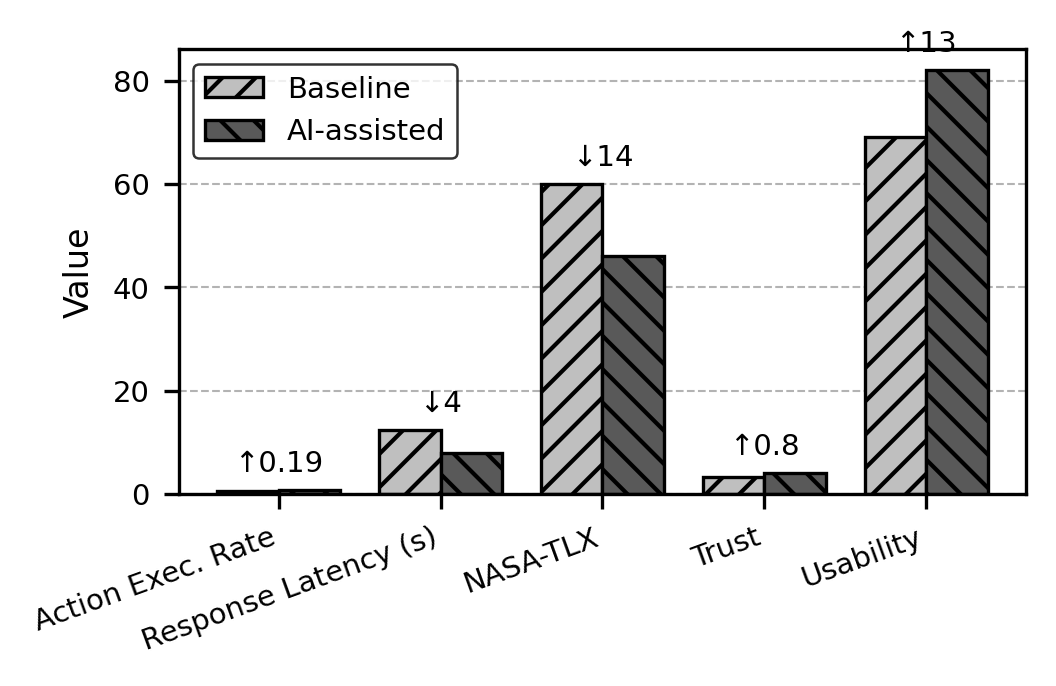
\includegraphics[width=0.9\linewidth]{fig_workload_trust_summary.png}
%DIFDELCMD <         \caption{Comparison of cognitive workload, trust, and usability between baseline and AI-assisted conditions. Lower NASA--TLX scores indicate reduced cognitive workload, while higher trust and usability scores indicate improved subjective evaluations.}
%DIFDELCMD <         \label{fig:workload_trust_summary}
%DIFDELCMD <     \end{figure}
%DIFDELCMD < %%%
\DIFdelend \DIFaddbegin \DIFadd{\textbf{Usability} was measured after each condition with the System Usability Scale (SUS) \cite{Brooke1996}: ten 5-point items with standard scoring to 0--100 (higher is better). The overall SUS scores in the study records exceed the scores recomputed from the item responses by a constant 2.8 points in every baseline record and 4.7 points in every AI-assisted record (recomputed means 65.7 and 77.0), and item consistency was low ($\alpha = .49$ and $.44$). We report the logged overall score as the primary SUS result (Table~\ref{tab:primary}) and the recomputed score as a robustness check (Section~\ref{sec:res_sub}).
}\DIFaddend 

    \DIFdelbegin \subsection{\DIFdel{Task Performance Outcomes}}
%DIFAUXCMD
\addtocounter{subsection}{-1}%DIFAUXCMD
%DIFDELCMD < 

%DIFDELCMD <     %%%
\DIFdel{The performance in the execution of the objective task was enhanced with the help of AI, as shown in Fig. ~\ref{fig:workload_trust_summary}. }\DIFdelend \DIFaddbegin \DIFadd{\textbf{Qualitative observations.} Post-task interview comments were summarized into themes but not systematically coded (prevalence not recorded); they are informal observations, and we do not describe the study as mixed-method.
}\DIFaddend 

    \DIFdelbegin \DIFdel{It is observed that the rate of action execution was enhanced by a small amount, from 0.55 in the baseline scenario to 0.74 in }\DIFdelend \DIFaddbegin \subsection{\DIFadd{Statistical Analysis}}
    \DIFadd{All analyses used the participant as the unit of analysis (paired design, $n=52$); trial-level outcomes were aggregated to one value per participant and condition (AER is the proportion of correct trials, latency the mean over the 10 trials). H1 (AER) is }\DIFaddend the \DIFaddbegin \DIFadd{primary hypothesis; H2--H4 (latency, NASA--TLX, trust, SUS) form the secondary family. For every outcome we report the condition means and SDs, the mean paired difference (}\DIFaddend AI-assisted \DIFdelbegin \DIFdel{scenario. This shows that the number of actions executed was higher in the }\DIFdelend \DIFaddbegin \DIFadd{minus baseline) with its 95\% confidence interval (Student's $t$), the two-sided paired $t$-test ($df=51$), and the standardized paired effect size $d_z$ \cite{Lakens2013} (mean difference divided by the SD of the differences) with a 95\% percentile-bootstrap CI (10}{\DIFadd{,}}\DIFadd{000 resamples). The $p$ for H1 is unadjusted; the four secondary tests are Holm-adjusted, and subscale and item analyses are exploratory (Holm across nine tests). Normality of the paired differences was checked with the Shapiro--Wilk test; it was rejected only for the trust outcomes ($p \leq .001$), and the Wilcoxon signed-rank test gave the same conclusions for those and all other outcomes. Because AER is bounded and based on 10 binary trials, we confirmed it with a trial-level logistic model estimated by generalized estimating equations (exchangeable correlation, clustered by participant); because trial-level latency is right-skewed, we confirmed it with a linear mixed model on log-latency with a participant random intercept. Order effects were tested with the standard two-sequence crossover approach (treatment-by-order interaction: Welch $t$ on the paired differences of the sequence groups; carry-over: participant sums compared between groups). The escalated vs.\ non-escalated comparison is descriptive only, because the two sets are not comparable. Exploratory analyses classed errors as under- or over-responses (options ordered from monitor to recommend evacuation; paired participant-level rates, unadjusted $t$-tests) and compared the reference-action distributions of the two conditions with a trial-level $\chi^2$ test as an indication of comparable content. All analyses used the script provided with the paper.
    }\subsection{\DIFadd{Data and Code Availability}}
    \label{sec:data}
    \DIFadd{The anonymized participant, questionnaire, and trial-level records (52 participants $\times$ 2 conditions $\times$ 10 trials) and the analysis scripts that produce every number, table, and figure in Section~\ref{sec:results} are distributed with the paper (folders \texttt{data/} and \texttt{analysis/}), restricted to the reproduction of this study. Trial behavior and response times were recorded automatically (latency is the difference between display and response timestamps, at 0.1~s resolution), and questionnaires were collected with Qualtrics as integer 1--5 responses. The overall SUS score in the questionnaire file is not the standard score of the stored items: it exceeds the recomputed score by exactly 2.8 points in all 52 baseline records and by exactly 4.7 points in all 52 }\DIFaddend AI-assisted \DIFdelbegin \DIFdel{scenario}\DIFdelend \DIFaddbegin \DIFadd{records. It is the value exported from Qualtrics, whose scoring configuration is not documented, so we report both scores (Section~\ref{sec:res_sub}); the conclusion is the same}\DIFaddend .

    \DIFdelbegin \DIFdel{It is also observed that the response time was reduced.
The average response time was reduced from 12.3 seconds }\DIFdelend %DIF > ---------------------------------\input{./070-result}
    \DIFaddbegin \section{\DIFadd{Results}}
    \label{sec:results}
    \DIFadd{Table~\ref{tab:primary} reports all primary and secondary outcomes. The sections below report each result with its statistics; interpretation is in Section~\ref{sec:discussion}.
}

    \begin{table*}[t]
        \caption{Primary and Secondary Outcomes: Baseline vs.\ AI-Assisted (ACHDF), $n=52$, Within-Subjects}
        \label{tab:primary}
        \centering
        \begin{tabular}{l c c c c c c}
            \toprule
            \textbf{Outcome} & \textbf{Baseline} & \textbf{AI-assisted} & \textbf{Difference [95\% CI]} & \textbf{$t(51)$} & \textbf{$p$} & \textbf{$d_z$ [95\% CI]} \\
            & M (SD) & M (SD) & (AI $-$ baseline) & & & \\
            \midrule
            \multicolumn{7}{l}{\emph{Primary (H1)}} \\
            AER (proportion) & 0.62 (0.19) & 0.81 (0.15) & 0.19 [0.14, 0.25] & 6.96 & $<.001$ & 0.96 [0.67, 1.36] \\
            \midrule
            \multicolumn{7}{l}{\emph{Secondary (H2--H4), Holm-adjusted}} \\
            Response latency (s) & 12.4 (0.8) & 8.1 (0.8) & $-$4.31 [$-$4.64, $-$3.97] & $-$25.98 & $<.001$ & $-$3.60 [$-$4.75, $-$2.90] \\
            NASA--TLX overall (0--100) & 59.8 (11.5) & 46.2 (9.3) & $-$13.6 [$-$17.8, $-$9.4] & $-$6.56 & $<.001$ & $-$0.91 [$-$1.30, $-$0.63] \\
            Trust overall (1--5) & 3.40 (0.57) & 4.20 (0.45) & 0.79 [0.61, 0.98] & 8.49 & $<.001$ & 1.18 [0.96, 1.53] \\
            SUS, as logged (0--100) & 68.5 (10.5) & 81.7 (8.6) & 13.2 [9.4, 16.9] & 7.08 & $<.001$ & 0.98 [0.74, 1.31] \\
            \bottomrule
            \multicolumn{7}{p{0.95\linewidth}}{\footnotesize M and SD are across the 52 participant-level values. Paired $t$-test, two-sided; $p$ for AER is unadjusted, $p$ for the four secondary outcomes is Holm-adjusted. $d_z$ = mean difference / SD of the differences; CIs by percentile bootstrap. Wilcoxon signed-rank tests gave $p<.001$ for every outcome. The SDs of latency are between-participant SDs of 10-trial means.}
        \end{tabular}
    \end{table*}

    \subsection{\DIFadd{Action Execution and Response Latency}}
    \label{sec:res_aer}
    \DIFadd{\textbf{H1.} The mean AER was 0.62 (SD 0.19) }\DIFaddend in the baseline \DIFdelbegin \DIFdel{scenario to 8.0 seconds }\DIFdelend \DIFaddbegin \DIFadd{condition and 0.81 (SD 0.15) }\DIFaddend in the AI-assisted \DIFdelbegin \DIFdel{scenario. The time was reduced by more than 4 seconds. This shows that the participants responded and executed actions in a better manner with the help of the AI system.
}%DIFDELCMD < 

%DIFDELCMD <     %%%
\subsection{\DIFdel{Cognitive Workload and Trust Outcomes}}
%DIFAUXCMD
\addtocounter{subsection}{-1}%DIFAUXCMD
\DIFdelend \DIFaddbegin \DIFadd{condition. The mean paired difference was $+0.19$ (95\% CI }[\DIFadd{0.14, 0.25}]\DIFadd{), $t(51)=6.96$, $p<.001$, $d_z=0.96$ (95\% CI }[\DIFadd{0.67, 1.36}]\DIFadd{), confirmed by the Wilcoxon signed-rank test ($p<.001$) and a trial-level logistic GEE model (odds ratio 2.61, 95\% CI }[\DIFadd{1.98, 3.45}]\DIFadd{, $p<.001$).
}\DIFaddend 

    \DIFdelbegin \DIFdel{A graphical representation of the results for workload, trust, and usability is shown in Fig.~\ref{fig:workload_trust_summary}.
    Cognitive workload, as assessed by NASA--TLX, was significantly lower in the AI-assisted condition than in the baseline condition. The total score on the NASA--TLX assessment dropped from around 60 }\DIFdelend \DIFaddbegin \DIFadd{\textbf{H2.} The mean response latency was 12.4~s (SD 0.8) in the baseline and 8.1~s (SD 0.8) in the AI-assisted condition, a difference of $-4.31$~s (95\% CI }[\DIFadd{$-4.64$, $-3.97$}]\DIFadd{), $t(51)=-25.98$, Holm-adjusted $p<.001$, $d_z=-3.60$ (95\% CI }[\DIFadd{$-4.75$, $-2.90$}]\DIFadd{). At the trial level, the median latency was 12.4~s (IQR 10.4--14.6) }\DIFaddend in the baseline \DIFdelbegin \DIFdel{condition to 46 }\DIFdelend \DIFaddbegin \DIFadd{and 7.9~s (IQR 6.6--9.7) }\DIFaddend in the AI-assisted condition, \DIFdelbegin \DIFdel{a reduction of 14 points. This is a clear indication of reduced workload in the AI-assisted condition}\DIFdelend \DIFaddbegin \DIFadd{and a mixed model on log-latency estimated a ratio of 0.65 (95\% CI }[\DIFadd{0.63, 0.67}]\DIFadd{). Because participants' mean latencies varied little within each condition (SD about 0.8~s) and did not correlate across conditions ($r=-.09$), $d_z$ is very large; we therefore interpret the raw difference (about 4~s) rather than $d_z$}\DIFaddend .
\DIFdelbegin \DIFdel{The NASA--TLX scores are summarized in Table~\ref{tab:workload}.Trust ratings were higher for the AI-assisted system. The average trust score was higher in the }\DIFdelend \DIFaddbegin 

    \DIFadd{\textbf{Wrong versus late actions.} Every unsuccessful trial is a wrong-action trial (198 of 520 baseline trials, 38.1\%; 99 of 520 }\DIFaddend AI-assisted \DIFdelbegin \DIFdel{condition, increasing from around 3.2 in the baseline condition to 4.0 on a 5-point scale in the }\DIFdelend \DIFaddbegin \DIFadd{trials, 19.0\%). Within each condition, wrong and correct trials had almost the same mean latency (baseline: 12.6~s vs.\ 12.3~s; }\DIFaddend AI-assisted\DIFdelbegin \DIFdel{condition, indicating that the system was perceived as more trustworthy and appropriate in its guidance.Usability was also higher in the }\DIFdelend \DIFaddbegin \DIFadd{: 8.1~s vs.\ 8.1~s), so slow responses do not account for the failures, and no speed--accuracy trade-off is visible. As a hypothetical sensitivity analysis (the actual scoring applied no cutoff), requiring a trial to be correct \emph{and} completed within a cutoff $T$ gives baseline vs.\ }\DIFaddend AI-assisted \DIFdelbegin \DIFdel{condition.
The system usability scores increased from around 69 to 82, a jump of 13 points, indicating that the participants found the }\DIFdelend \DIFaddbegin \DIFadd{AER of 0.14 vs.\ 0.64 at $T=10$~s, 0.29 vs.\ 0.77 at 12~s, and 0.50 vs.\ 0.81 at 15~s (all paired differences $p<.001$); the advantage grows as $T$ becomes stricter, reflecting the shorter latencies.
}

    \DIFadd{\textbf{Direction of errors and comparability of content (exploratory).} Ordering the options from monitor to recommend evacuation, 54.5\% of errors in both conditions (108 of 198 baseline, 54 of 99 }\DIFaddend AI-assisted\DIFdelbegin \DIFdel{system interface easier and more effective to use.The trust and usability scores are summarized in Table~\ref{tab:trust_usability}.}\DIFdelend \DIFaddbegin \DIFadd{) were under-responses, i.e., a less severe action than the reference; the rest were over-responses. The mean distance from the reference option was about two steps in both conditions (2.02 and 2.05). Both kinds of error were less frequent with AI support: per participant, under-responses fell from 0.21 to 0.10 of trials ($-0.10$, 95\% CI }[\DIFadd{$-0.15$, $-0.06$}]\DIFadd{, $t(51)=-5.01$, $d_z=-0.69$) and over-responses from 0.17 to 0.09 ($-0.09$, 95\% CI }[\DIFadd{$-0.13$, $-0.05$}]\DIFadd{, $t(51)=-4.21$, $d_z=-0.58$; both unadjusted, $p<.001$), so errors were not shifted toward one side. The ordering is a working assumption, and the logs do not say which errors would be costlier. As an indication of comparable content, the reference actions were similarly distributed across conditions (trial-level $\chi^2(4)=9.16$, $p=.057$, Cram\'er's $V=.09$), with somewhat more shelter-in-place reference trials in the baseline (28\% vs.\ 21\%); because stimulus content is not stored, this is the only available difficulty-control check.
}\DIFaddend 

    \DIFdelbegin \subsection{\DIFdel{Effects of Uncertainty-Aware Escalation}}
    %DIFAUXCMD
\addtocounter{subsection}{-1}%DIFAUXCMD
\DIFdel{When the uncertainty thresholds were exceeded, human-in-the-loop escalation occurred. In such cases, the participants appropriately deferred their decisions until further confirmation or clarification was available. No increase in inappropriate use of the system recommendations in high-uncertainty cases was observed. The results comparing escalated and non-escalated cases are presented in Table~\ref{tab:escalation}. These results show that uncertainty-aware escalation maintained system effectiveness while preventing over-reliance on the system. }\DIFdelend \DIFaddbegin \subsection{\DIFadd{Workload, Trust, and Usability}}
    \label{sec:res_sub}
    \DIFadd{Table~\ref{tab:subscales} gives the trust item results.
}\DIFaddend 

    \DIFdelbegin \subsection{\DIFdel{Qualitative Observations}}
%DIFAUXCMD
\addtocounter{subsection}{-1}%DIFAUXCMD
\DIFdelend \DIFaddbegin \DIFadd{\textbf{H3.} The overall NASA--TLX score was 59.8 (SD 11.5) in the baseline and 46.2 (SD 9.3) in the AI-assisted condition, a difference of $-13.6$ points (95\% CI }[\DIFadd{$-17.8$, $-9.4$}]\DIFadd{), $t(51)=-6.56$, Holm-adjusted $p<.001$, $d_z=-0.91$ (95\% CI }[\DIFadd{$-1.30$, $-0.63$}]\DIFadd{). All six subscales were lower in the AI-assisted condition, from $-9.7$ points for frustration ($d_z=-0.45$) to $-17.4$ for performance ($d_z=-0.80$), all Holm-adjusted $p \leq .002$ (full subscale table in the analysis output distributed with the paper).
}\DIFaddend 

    \DIFdelbegin \DIFdel{The post-task interviews allowed for qualitative analysis of }\DIFdelend \DIFaddbegin \DIFadd{\textbf{H4.} The overall trust score was 3.40 (SD 0.57) in the baseline and 4.20 (SD 0.45) in the AI-assisted condition, a difference of $+0.79$ (95\% CI }[\DIFadd{0.61, 0.98}]\DIFadd{), $t(51)=8.49$, Holm-adjusted $p<.001$, $d_z=1.18$ (95\% CI }[\DIFadd{0.96, 1.53}]\DIFadd{); the paired differences were not normally distributed (Shapiro--Wilk $p=.001$), and the Wilcoxon test gave the same conclusion ($p<.001$). The SUS score was 68.5 (SD 10.5) in the baseline and 81.7 (SD 8.6) in the AI-assisted condition, a difference of $+13.2$ points (95\% CI }[\DIFadd{9.4, 16.9}]\DIFadd{), $t(51)=7.08$, Holm-adjusted $p<.001$, $d_z=0.98$ (95\% CI }[\DIFadd{0.74, 1.31}]\DIFadd{). With the SUS recomputed from the item responses (65.7 vs.\ 77.0), }\DIFaddend the \DIFdelbegin \DIFdel{participants'experiences. Participants often pointed out that the AI recommendations diminished the need for cross-referencing between different information sources.Some participants also emphasized the importance of having explicit uncertainty indicators to guide their confidence in decisions.
Some qualitative findings are presented in Table~\ref{tab:qualitative}. These findings supplement the quantitative findings by providing a glimpse into the participants' experiences with the system during decision-making tasks. To mitigate the potential for a Type~I error due to multiple comparisons, all primary hypotheses were defined a~priori, and consistent performance patterns were verified across different objective and subjective measures}\DIFdelend \DIFaddbegin \DIFadd{difference was $+11.3$ points (95\% CI }[\DIFadd{7.5, 15.0}]\DIFadd{), $t(51)=6.06$, $p<.001$, $d_z=0.84$}\DIFaddend .

    \DIFdelbegin %DIFDELCMD < \begin{table}[t]
%DIFDELCMD <         \caption{Cognitive Workload and Trust Scores}
%DIFDELCMD <         \label{tab:workload_trust}
%DIFDELCMD <         \centering
%DIFDELCMD <         \begin{tabular}{l c c}
%DIFDELCMD <             \hline
%DIFDELCMD <             Measure & Baseline & AI-Assisted \\
%DIFDELCMD <             \hline
%DIFDELCMD <             NASA--TLX & 59.8 & 46.2 \\
%DIFDELCMD <             Trust score & 3.4 & 4.2 \\
%DIFDELCMD <             \hline
%DIFDELCMD <         \end{tabular}
%DIFDELCMD <     \end{table}
%DIFDELCMD < 

%DIFDELCMD <     \begin{table}[t]
%DIFDELCMD <         \caption{Action execution and response latency (controlled study)}
%DIFDELCMD <         \label{tab:action_latency}
%DIFDELCMD <         \centering
%DIFDELCMD <         \begin{tabular}{lcc}
%DIFDELCMD <             \toprule
%DIFDELCMD <             \textbf{Metric} & \textbf{Baseline} & \textbf{AI-assisted} \\
%DIFDELCMD <             \midrule
%DIFDELCMD <             Action Execution Rate (AER) & 0.62 & 0.81 \\
%DIFDELCMD <             Response Latency (s) & 12.4 & 8.1 \\
%DIFDELCMD <             Effect size (Cohen's $d$) & \multicolumn{2}{c}{0.86} \\
%DIFDELCMD <             \bottomrule
%DIFDELCMD <         \end{tabular}
%DIFDELCMD <     \end{table}
%DIFDELCMD < 

%DIFDELCMD <     \begin{table}[t]
%DIFDELCMD <         \caption{Workload, trust, and usability outcomes (controlled study)}
%DIFDELCMD <         \label{tab:workload_trust}
%DIFDELCMD <         \centering
%DIFDELCMD <         \begin{tabular}{lcc}
%DIFDELCMD <             \toprule
%DIFDELCMD <             \textbf{Metric} & \textbf{Baseline} & \textbf{AI-assisted} \\
%DIFDELCMD <             \midrule
%DIFDELCMD <             NASA--TLX (overall) & 59.8 & 46.2 \\
%DIFDELCMD <             Trust (Likert-type composite) & 3.4 & 4.2 \\
%DIFDELCMD <             Usability score & 68.5 & 81.7 \\
%DIFDELCMD <             \bottomrule
%DIFDELCMD <         \end{tabular}
%DIFDELCMD <     \end{table}
%DIFDELCMD < 

%DIFDELCMD <     \begin{table}[t]
%DIFDELCMD <         \caption{Outcomes by uncertainty-aware escalation status}
%DIFDELCMD <         \label{tab:escalation}
%DIFDELCMD <         \centering
%DIFDELCMD <         \begin{tabular}{lcc}
%DIFDELCMD <             \toprule
%DIFDELCMD <             \textbf{Metric} & \textbf{No escalation} & \textbf{Escalation triggered} \\
%DIFDELCMD <             \midrule
%DIFDELCMD <             Appropriate deferral rate & 0.21 & 0.47 \\
%DIFDELCMD <             Inappropriate reliance rate & 0.18 & 0.09 \\
%DIFDELCMD <             \bottomrule
%DIFDELCMD <         \end{tabular}
%DIFDELCMD <     \end{table}
%DIFDELCMD < 

%DIFDELCMD <     \begin{table}[t]
%DIFDELCMD <         \caption{Qualitative themes from post-task interviews}
%DIFDELCMD <         \label{tab:qualitative}
%DIFDELCMD <         \centering
%DIFDELCMD <         \begin{tabular}{p{0.27\linewidth}p{0.64\linewidth}}
%DIFDELCMD <             \toprule
%DIFDELCMD <             \textbf{Theme} & \textbf{Illustrative observation (paraphrased)} \\
%DIFDELCMD <             \midrule
%DIFDELCMD <             Reduced context switching & Recommendations decreased the need to cross-reference multiple sources. \\
%DIFDELCMD <             Uncertainty cue usefulness & Participants used uncertainty cues to decide when to defer or seek confirmation. \\
%DIFDELCMD <             Accountability and control & Human override improved perceived safety and responsibility. \\
%DIFDELCMD <             \bottomrule
%DIFDELCMD <         \end{tabular}
%DIFDELCMD <     \end{table}
%DIFDELCMD < %%%
\DIFdelend \DIFaddbegin \begin{table*}[t]
        \caption{Exploratory Analysis of the Trust Items, $n=52$ (Holm-Adjusted Across the Nine Subscale and Item Tests)}
        \label{tab:subscales}
        \centering
        \begin{tabular}{l c c c c c c}
            \toprule
            \textbf{Measure} & \textbf{Baseline} & \textbf{AI-assisted} & \textbf{Difference [95\% CI]} & \textbf{$t(51)$} & \textbf{$p$} & \textbf{$d_z$ [95\% CI]} \\
            & M (SD) & M (SD) & (AI $-$ baseline) & & & \\
            \midrule
            \multicolumn{7}{l}{\emph{Trust items (1--5)}} \\
            Perceived reliability & 3.38 (0.69) & 4.17 (0.73) & 0.79 [0.55, 1.02] & 6.70 & $<.001$ & 0.93 [0.62, 1.36] \\
            Perceived predictability & 3.44 (0.73) & 4.13 (0.66) & 0.69 [0.42, 0.96] & 5.20 & $<.001$ & 0.72 [0.50, 0.99] \\
            Perceived appropriateness & 3.38 (0.87) & 4.23 (0.55) & 0.85 [0.59, 1.11] & 6.51 & $<.001$ & 0.90 [0.67, 1.24] \\
            \bottomrule
        \end{tabular}
    \end{table*}
\DIFaddend 

    \DIFdelbegin \subsection{\DIFdel{Mechanism and Multi-layer Analysis Under ACHDF}}
    %DIFAUXCMD
\addtocounter{subsection}{-1}%DIFAUXCMD
%DIFDELCMD < \label{sec:results_mechanism}
%DIFDELCMD < %%%
\DIFdelend \DIFaddbegin \subsection{\DIFadd{Order and Carry-Over Effects}}
    \label{sec:res_order}
    \DIFadd{Neither the treatment-by-order interaction nor the carry-over test was significant for any outcome (all $p \geq .07$). The AER difference was $+0.23$ in participants who used the AI-assisted condition first and $+0.15$ in those who used the baseline first (interaction $t=1.37$, $p=.18$; carry-over $p=.92$); interactions for latency ($p=.46$), NASA--TLX ($p=.62$), trust ($p=.07$), and SUS ($p=.14$) were likewise not significant. With 28 and 24 participants per sequence, these tests have limited power for moderate interactions, so a non-significant order effect does not prove that no carry-over occurred.
}\DIFaddend 

    \DIFdelbegin \DIFdel{In order to provide a structured understanding of how the achieved results were obtained at the behavioral level, we also analyzed the results through the prism of the Action-Centered Human--AI Decision Framework (ACHDF). This analysis does not include any new outcome measures but structures the existing results to reveal multi-layered patterns relevant to human action in the context of uncertainty.
    From the mechanism perspective, the increase in Action Execution Rate and the reduction in response latency (Table~\ref{tab:action_latency}, Fig.~\ref{fig:latency_distribution})may be considered a behavioral outcome of uncertainty-aware function allocation, where the representation of uncertainty directly influences the allocation of decisions to the AI or human operators in terms of timing and correctness of action execution. At the level of error structure, uncertainty-aware escalation was found to influence participants’ responses in high-uncertainty scenarios. As depicted in Table~\ref{tab:escalation}, escalation was linked to increased appropriate deferral and reduced inappropriate reliance. These results indicate that uncertainty-aware escalation selectively mitigated failure modes related to hesitation and over-reliance, rather than indiscriminately increasing reliance on automation.
Lastly, qualitative results (Table~\ref{tab:qualitative}) and reductions in workload (Table~\ref{tab:workload}) indicate changes in decision processes in the }\DIFdelend \DIFaddbegin \subsection{\DIFadd{Escalated and Non-Escalated Trials (Descriptive)}}
    \label{sec:res_escalation}
    \DIFadd{Escalation was triggered in 150 of the 520 }\DIFaddend AI-assisted \DIFdelbegin \DIFdel{condition.Participants’ self-reported context switching and decision transitions align with reductions in response latency and workload. These findings on all three levels align with the premise of ACHDF: that human action in uncertain situations can be explained by the interaction of uncertainty-aware risk representation, bounded autonomy, calibrated trust, and cognitive workload management.
    Moreover, statistical tests for comparing the baseline and }\DIFdelend \DIFaddbegin \DIFadd{trials (28.8\%). Descriptively, non-escalated (370) and escalated (150) }\DIFaddend AI-assisted \DIFdelbegin \DIFdel{conditions revealed that the improvement in the rate of action execution and the reduction of latency while responding were statistically significant at a $p$ value of less than 0.01.
Differences observed for cognitive workload and trust levels, as measured by the NASA--TLX scale, were statistically significant at a $p$ value of less than 0.05}\DIFdelend \DIFaddbegin \DIFadd{trials had the same AER (0.81 vs.\ 0.81; baseline 0.62) and similar mean latency (8.0 vs.\ 8.5~s; baseline 12.4~s). These sets are not equivalent conditions: escalation is triggered by high uncertainty or criticality and explicitly prompts human review, so differences cannot be attributed causally to escalation. Deferral was flagged in 47.3\% of escalated, 18.4\% of non-escalated AI-assisted, and 11.3\% of baseline trials; per participant, the deferral rate was higher in the AI-assisted condition (0.27 vs.\ 0.11; difference $+0.15$, 95\% CI }[\DIFadd{0.11, 0.20}]\DIFadd{, $t(51)=6.92$, $d_z=0.96$). The logs contain neither the content nor the correctness of the AI recommendation, so rates of \emph{appropriate} deferral or \emph{inappropriate} reliance cannot be derived.
}



    \subsection{\DIFadd{Qualitative Observations}}
    \DIFadd{Informal interview comments (not coded; prevalence not recorded) described three recurring themes: recommendations reduced the need to cross-reference sources, participants used the uncertainty cues to decide when to defer or seek confirmation, and the ability to override improved perceived safety and responsibility}\DIFaddend .

    %----------------------------------------\input{./080-discussion}
\section{Discussion}
\DIFaddbegin \label{sec:discussion}
\DIFaddend This section interprets the \DIFdelbegin \DIFdel{empirical findings from a human--machine systems perspective and situates them within the broader literature on human--AI decision making. Rather than focusing on application-specific results, the discussion emphasizes generalizable insights for the design and evaluation of }\DIFdelend \DIFaddbegin \DIFadd{results at the level of the joint }\DIFaddend human--AI \DIFdelbegin \DIFdel{decision systems operating under uncertainty \cite{Bach2024Access,PerezCerrolaza2024CSUR,Lai2023FAccT,Yang2022THMSReview}. In particular, this work contributes to the core concerns of \textit{Human--Machine Systems} by explicitly linking uncertainty-aware function allocation to observable human action execution . By doing so, it extends classic HMS constructs---such as trust calibration, workload, and authority allocation---from internal cognitive or perceptual states to measurable behavioral outcomes. }\DIFdelend \DIFaddbegin \DIFadd{system \cite{Hollnagel2005JCS,Woods2006JCS}. Because the AI-assisted condition differed from the baseline in several features at once, statements about \emph{which} features produced the effects are hypotheses, not demonstrated causal pathways.
}\DIFaddend 

\DIFdelbegin \subsection{\DIFdel{Implications for Human--AI Decision Systems}}
%DIFAUXCMD
\addtocounter{subsection}{-1}%DIFAUXCMD
\DIFdel{The results show that human performance gain is not simply a function of the availability of }\DIFdelend \DIFaddbegin \subsection{\DIFadd{Action Execution in the Joint Human--AI System}}
\DIFadd{The AER was higher and the latency shorter in the AI-assisted condition, with large paired effects ($d_z=0.96$ for the AER), consistent with H1 and H2. Evaluating by action execution rather than prediction accuracy follows directly from the JCS perspective, whereas AI decision-support research is still dominated by accuracy and information quality \cite{Lai2023FAccT,Muller2022CHIWORK,Yang2022THMSReview}. Because the baseline offered no }\DIFaddend AI support, \DIFdelbegin \DIFdel{but also depends on how that support is organized to guide human action execution. By directly assessing action execution as an outcome measure, this research extends previous research that primarily tested decision support systems in terms of the accuracy of predictions or the quality of information \cite{Lai2023FAccT,Muller2022CHIWORK,Yang2022THMSReview}.
From a human--machine system perspective, action execution is the end result of human information processing that combines elements of perception, understanding, trust, and workload into system performance \cite{Hodgson2013THMS,Bach2024Access}. The increase in Action Execution Rate and the decrease in response latency indicate that human--AI systems are capable of significantly influencing human behavior when recommendations are presented in action format instead of risk format . This supports the move towards an outcome-oriented human--machine system research area where the effectiveness of AI support is determined in terms of human action instead of computer performance \cite{Lai2023FAccT,Yang2022THMSReview}. This research contributes to the Human--Machine Systems area by empirically connecting function allocation with uncertainty to human action execution.
The results demonstrate how design decisions in the architecture (bounded autonomy, uncertainty representation, and escalation strategies) map to behavioral phenomena, thus closing the theoretical-practice divide in human factors theory and human--AI system design \cite{Bach2024Access,Assaad2023TAS,Zhang2022THMS}.In this respect, the Action-Centered Human--AI Decision Framework (ACHDF)may also be used as an analytical tool for identifying failure modes in existing human--AI systems, aside from the system examined in this research \cite{Yang2022THMSReview,Lai2023FAccT}.
}\DIFdelend \DIFaddbegin \DIFadd{the comparison shows the benefit of integrated ACHDF support over a dashboard, not how much is due to the structure of the support rather than the availability of AI support, which would require a condition with unstructured AI recommendations.
}\DIFaddend 

\DIFdelbegin \subsection{\DIFdel{Trust Calibration and Automation Bias}}
%DIFAUXCMD
\addtocounter{subsection}{-1}%DIFAUXCMD
\DIFdel{The main contribution of this research is in the way it approaches the issue of trust calibration. The findings show that the more trust participants had in the AI-assisted system, the more this did not translate to automation bias. Instead, participants displayed appropriate trust }\DIFdelend \DIFaddbegin \DIFadd{Several features could explain the improvement: the presence of a recommendation, its action-oriented phrasing, the uncertainty and criticality cues, and escalation. The design does not separate them, so we cannot conclude that presenting recommendations }\DIFaddend in \DIFdelbegin \DIFdel{the system and delayed action in situations of high uncertainty and appropriate use of human-in-the-loop escalation mechanisms \cite{Raji2019AIES,Raji2022CACM,Weidinger2022FAccT}. The findings demonstrate the effect of }\DIFdelend \DIFaddbegin \DIFadd{an action format rather than a risk format caused the improvement; a factorial design that varies the format while holding the other features constant is needed (Section~\ref{sec:limitations}). The AER gain stems from fewer wrong actions, not fewer late ones (Section~\ref{sec:res_aer}), but why the AI-assisted condition was more accurate is not identified.
}

\subsection{\DIFadd{Framework-Based Interpretation of the Results}}
\label{sec:interpretation}
\DIFadd{The following reading organizes the observed results along the ACHDF layers. It does not test the proposed mechanisms. \emph{Action level:} the higher AER and lower latency (Table~\ref{tab:primary}) are consistent with the idea that }\DIFaddend uncertainty-aware \DIFdelbegin \DIFdel{design and }\DIFdelend \DIFaddbegin \DIFadd{adaptation of support helps operators move from risk interpretation to action. \emph{Error-structure level:} deferral was flagged more often in escalated than in non-escalated AI-assisted trials (47\% vs.\ 18\%) while the AER was the same (0.81; Section~\ref{sec:res_escalation}); because escalation is triggered by uncertainty and criticality and itself prompts review, this pattern is descriptive, and, without the content or correctness of the AI advice, it is compatible with but does not demonstrate a protective effect of escalation against over-reliance.
}

\DIFadd{\textbf{Workload as a possible explanation.} Lower workload is a plausible contributor to better action execution. The NASA--TLX, however, is a retrospective, subjective, condition-level measure, and we did not test whether the workload reduction explains the AER improvement; with one measurement per condition, a mediation analysis could not separate workload from the other differences between conditions. This link is therefore a possible explanatory mechanism, not a demonstrated pathway.
}

\subsection{\DIFadd{Trust and Automation Bias}}
\DIFadd{Perceived trust was higher in the AI-assisted condition ($d_z=1.18$), although the three trust items had low internal consistency ($\alpha = .46$--$.61$). Higher trust is not \emph{calibrated} trust, which requires that reliance match the actual reliability of the advice \cite{Lee2004} and so needs trial-by-trial data on the correctness of }\DIFaddend the \DIFdelbegin \DIFdel{use of design constraints in avoiding typical automation failure modes. In this way, the system did not provide false confidence to the participants. These findings validate human factors theories emphasizing the importance of trust calibration in effective human--AI cooperation and provide evidence of this in design \cite{Hodgson2013THMS,Bach2024Access}. These results provide empirical support for long-held theoretical assertions in human--machine systems research that }\DIFdelend \DIFaddbegin \DIFadd{AI's recommendations; the greater deferral in escalated trials is not evidence of calibration either, because escalation itself prompts review. We make no claim that ACHDF calibrates trust. Similarly, }\DIFaddend automation bias can be \DIFdelbegin \DIFdel{reduced by incorporating uncertainty representation and human-in-the-loop escalation. Contrary to the potential for increasing over-reliance, the proposed design facilitated calibrated trust by aligning perceived system confidence with actual uncertainty \cite{Miller2019XRDS,Weidinger2022FAccT,Lai2023FAccT}}\DIFdelend \DIFaddbegin \DIFadd{assessed directly only on trials in which the AI's advice is wrong, by measuring how often participants accept it \cite{Parasuraman2010}. The logs do not record the AI recommendation or its correctness, so behavior on erroneous recommendations could not be analyzed, and the study cannot show whether ACHDF reduces automation bias}\DIFaddend .

\DIFdelbegin %DIFDELCMD < \begin{table}[t]
%DIFDELCMD <         \caption{Design Implications for Human--AI Decision Systems}
%DIFDELCMD <         \label{tab:design_implications}
%DIFDELCMD <         \centering
%DIFDELCMD <         \begin{tabular}{l l}
%DIFDELCMD <             \hline
%DIFDELCMD <             Finding & Design Implication \\
%DIFDELCMD <             \hline
%DIFDELCMD <             Higher AER & Action-oriented recommendations \\
%DIFDELCMD <             Reduced workload & Information structuring \\
%DIFDELCMD <             Calibrated trust & Explicit uncertainty \\
%DIFDELCMD <             \hline
%DIFDELCMD <         \end{tabular}
%DIFDELCMD <     \end{table}
%DIFDELCMD <     

%DIFDELCMD < %%%
\DIFdelend \subsection{\DIFdelbegin \DIFdel{Design Implications for High-Risk Domains}\DIFdelend \DIFaddbegin \DIFadd{Ecological Validity of Escalation}\DIFaddend }
\DIFdelbegin \DIFdel{Although the empirical studywas carried out in the context of disaster response, }\DIFdelend \DIFaddbegin \DIFadd{In the study, participants could defer a decision when the system escalated. In real time-critical emergencies, deferral may not be feasible or may itself be costly: an operator may have to act on uncertain information before an evacuation window closes. The higher deferral in escalated trials (Section~\ref{sec:res_escalation}) was possible only because deferral was available, and since reliance on erroneous advice could not be measured, }\DIFaddend the \DIFdelbegin \DIFdel{design principles and results can be generalized to other high-risk domains such as healthcare, transportation, and industrial safety, where the cost of inappropriate or delayed response is high, and complete automation is not always feasible or desirable \cite{PerezCerrolaza2024CSUR,Rao2024IJDRS,Rokhideh2025IJDRS,Birkmann2013NatHazards}. Similar action-centered constraints and explainability considerations also arise in cyber-physical production and Industry~4.0 security decision support \cite{Farhan2025TCE}.
The findings of the study indicate that human--AI decision-making systems should be designed in such a way that they }\DIFdelend \DIFaddbegin \DIFadd{study provides no direct evidence that escalation reduced over-reliance or automation bias. Any such benefit that operates through deferral may not carry over to settings where deferral is constrained; future studies should assign explicit costs to deferral and include forced-choice conditions.
}

\subsection{\DIFadd{Design Implications}}
\DIFadd{Within the evaluated task, the results suggest that decision support may benefit from }\DIFaddend (1) \DIFdelbegin \DIFdel{model }\DIFdelend \DIFaddbegin \DIFadd{representing }\DIFaddend uncertainty explicitly, (2) \DIFdelbegin \DIFdel{provide }\DIFdelend \DIFaddbegin \DIFadd{providing }\DIFaddend action guidance rather than \DIFaddbegin \DIFadd{only }\DIFaddend passive information display, and (3) \DIFdelbegin \DIFdel{allocate decision authority dynamically }\DIFdelend \DIFaddbegin \DIFadd{adapting the level and form of support to uncertainty and criticality }\DIFaddend through human-in-the-loop escalation \DIFdelbegin \DIFdel{\cite{Assaad2023TAS,Zhang2022THMS,Bach2024Access}.
Based on the Human--Machine Systems model, the results of the current study imply that effective decision systems with AI assistance need to be based on the concepts of bounded autonomy and decision authority allocation, as well as uncertainty-aware interaction.
These concepts are not limited to the disaster response domain and are generally applicable to a wide variety of safety-critical human--machine systems with AI assistance \cite{Yang2022THMSReview,PerezCerrolaza2024CSUR}.
The observed effects of the described phenomenon are not domain-specific but rather general mechanisms of human--machine interaction, which are relevant to any }\DIFdelend \DIFaddbegin \DIFadd{while leaving final authority with the human \cite{Assaad2023TAS,Zhang2022THMS,Bach2024Access,Parasuraman2000LOA}. Each finding has several candidate explanations (e.g., higher AER: action-oriented recommendations; lower NASA--TLX: consolidated information structuring; higher trust: explicit uncertainty and criticality cues), so each implication should be tested individually, and transfer to other }\DIFaddend safety-critical \DIFdelbegin \DIFdel{decision system \cite{Bach2024Access,Hodgson2013THMS}.
In general, the current study contributes to the broader area of human--machine systems by showing the benefits of the application of human-centered AI decision systems with awareness of uncertainty for the execution of actions without compromising safety and accountability \cite{Lai2023FAccT,Yang2022THMSReview}. The design implications that are critical based on the findings are presented in Table~\ref{tab:design_implications}.
        In providing insight into the manner in which architectural design translates into behavioral outcomes, the results contribute to the domain of human machine systems with respect to trust calibration and cognitive ergonomics. }\DIFdelend \DIFaddbegin \DIFadd{domains \cite{PerezCerrolaza2024CSUR} has not been tested here.
}\DIFaddend 

    %---------------------------------\input{./090-futurework}
    \DIFdelbegin \section{\DIFdel{Limitations and Future Work}}
    %DIFAUXCMD
\addtocounter{section}{-1}%DIFAUXCMD
\DIFdel{The research has several limitations, which also point to potential directions for future research in similar studies. Although the research provides valuable data in terms of the effectiveness of the human--AI system in decision-making, it must be considered in relation to the limitations of this research.
        }%DIFDELCMD < 

%DIFDELCMD <     %%%
\subsection{\DIFdel{Generalization}}
    %DIFAUXCMD
\addtocounter{subsection}{-1}%DIFAUXCMD
\DIFdel{The study has conducted an empirical evaluation using a set of decision scenarios in relation to a disaster response scenario. Although this scenario is representative of a high-stakes decision-making scenario in which there is considerable uncertainty, future research can be conducted to evaluate the generalization of the proposed design principles across diverse domains and professionals in which there is considerable expertise. }\DIFdelend \DIFaddbegin \section{\DIFadd{Limitations and Future Work}}
    \label{sec:limitations}
\DIFaddend 

    \DIFdelbegin \subsection{\DIFdel{Long-Term Trust Effects}}
    %DIFAUXCMD
\addtocounter{subsection}{-1}%DIFAUXCMD
\DIFdel{The research has focused on the short-term effects of human--AI systems.
        Although it is recognized that the study has focused on the short term, it is anticipated that the long-term effects of trust will be considerable in relation to operators' exposure to the system and its behavior in relation to uncertainty escalation.
}\DIFdelend \DIFaddbegin \subsection{\DIFadd{Bundled Intervention}}
    \DIFadd{The study estimates the effect of the integrated ACHDF configuration and cannot attribute effects to individual components (uncertainty display, action format, escalation, guardrails); future work should use factorial or ablation designs.
}\DIFaddend 

    \DIFdelbegin \subsection{\DIFdel{Extension of the Research Beyond Disaster Response}}
    %DIFAUXCMD
\addtocounter{subsection}{-1}%DIFAUXCMD
\DIFdel{The research has focused on the domain of disaster response and has recognized this domain as effective in relation to testing systems in a high-stakes scenario . Although the domain is recognized as effective in relation to testing systems in }\DIFdelend \DIFaddbegin \subsection{\DIFadd{Trust Calibration and Automation Bias}}
    \DIFadd{Trust was measured as }\DIFaddend a \DIFdelbegin \DIFdel{high-stakes scenario, future research can be conducted to extend the system beyond this domain to other high-stakes domains such as medical systems and traffic management systems}\DIFdelend \DIFaddbegin \DIFadd{condition-level attitude, and behavior on erroneous AI recommendations was not analyzed, so neither calibration nor automation bias could be assessed; future studies should include incorrect advice and measure reliance trial by trial.
}

    \subsection{\DIFadd{Domain and Population Generalizability}}
    \DIFadd{The evaluation used only simulated disaster-response scenarios. Participants were not required to have domain expertise and were not specifically emergency-management professionals; trained operators may rely less on recommendations, use different heuristics, or experience different workload. Generalization to other domains (e.g., medical triage, autonomous driving supervision, traffic management) and to professional operators remains future work: ACHDF addresses a class of decision ecologies with high uncertainty, asymmetric error costs, time pressure, and human accountability, but time scales, operator expertise, and regulatory constraints differ substantially across domains, and any transfer is a hypothesis.
}

    \subsection{\DIFadd{Reporting and Analysis Limitations}}
    \label{sec:lim_reporting}
    \DIFadd{The statistics were computed from the anonymized study logs, which resolved most reporting gaps of the earlier version. The following limitations remain:
    }\begin{itemize}
        \item \DIFadd{\emph{Scoring of the primary outcome.} How the reference action of each trial was determined, in particular whether it was fixed independently of the AI recommendation, is not documented, and no per-trial time limit or time-out flag is recorded. The AER is a correct-action rate, and the time-cutoff analysis is hypothetical.
        }\item \DIFadd{\emph{Scenario identity and difficulty.} The reference action recorded for a label S01--S10 differs across participants, and for the same participant and label it matched between conditions in only 18\% of the pairs, so identical scenarios across conditions cannot be verified. The reference-action distribution differed slightly between conditions ($\chi^2(4)=9.2$, $p=.057$), and per-trial uncertainty and criticality were not logged, so the scenario mix could not be used as a covariate.
        }\item \DIFadd{\emph{Task and materials.} Per-trial stimulus values, the per-trial time limit, the total training duration and any pass criterion, and screenshots of the study interface are not documented; the interface figure is a reconstructed illustration. This limits reproducibility.
        }\item \DIFadd{\emph{System implementation.} The risk model, thresholds, and guardrails are described in Sections~\ref{sec:risk} and~\ref{sec:guardrails} for the study prototype (the open reference implementation). The model's calibration was not evaluated; $\tau_u$, $\tau_c$, and the criticality scale are not documented; and the prototype has no escalation branch. Escalation was pre-assigned in the scenario design (the values used are not documented), so the study evaluates the escalate presentation but not the run-time threshold logic of Algorithm~\ref{alg:escalation}.
        }\item \DIFadd{\emph{Measures.} The trust items have no published validation and low internal consistency ($\alpha = .46$--$.61$); the ten SUS items also had low consistency ($\alpha = .44$--$.49$), and the logged SUS scores exceed the recomputed scores by a constant 2.8 (baseline) and 4.7 (AI-assisted) points with an undocumented scoring configuration. The conclusion is the same under both scores, but absolute SUS values should not be compared with benchmarks. Questionnaire responses may reflect demand effects, as participants knew which condition was the proposed system. The interviews were not systematically coded.
        }\item \DIFadd{\emph{Ethics.} The study has no IRB approval or exemption number, because the author's institutional IRB advised that it is outside the scope of review (Section~\ref{sec:participants}); informed consent and anonymization are the safeguards that can be reported.
    }\end{itemize}
    \DIFadd{Future studies should preregister their analyses, log the AI recommendation and its correctness, the scenario content, and the uncertainty and criticality of each trial, share trial-level data and materials, and examine longer-term trust and reliance in field studies, since this study captured only short-term effects within a single session}\DIFaddend .

    %-------------------------------\input{./092-conclusion}
\section{Conclusion}
This \DIFdelbegin \DIFdel{work evaluated }\DIFdelend \DIFaddbegin \DIFadd{paper presented ACHDF, }\DIFaddend an action-centered human--AI decision \DIFdelbegin \DIFdel{system for disaster-risk contexts and showed that an ACHDF-based, }\DIFdelend \DIFaddbegin \DIFadd{framework that instantiates the joint cognitive systems perspective for disaster-response decision support. ACHDF combines }\DIFaddend uncertainty-aware \DIFdelbegin \DIFdel{architecture improves action execution (higher AER and lower response latency ) while reducing cognitive workload (NASA--TLX)}\DIFdelend \DIFaddbegin \DIFadd{risk estimation, guardrailed recommendations, and uncertainty- }\DIFaddend and \DIFdelbegin \DIFdel{supporting calibrated trust without increasing automation bias. By empirically linking uncertainty-aware function allocation, guardrailed recommendations, and human-in-the-loop escalation to observable action execution, the paper advances core concerns of human--machine systems and provides transferable design principles for other safety-critical decision ecologies}\DIFdelend \DIFaddbegin \DIFadd{criticality-triggered escalation, while the human keeps final decision authority. In a within-subjects study with 52 participants, the integrated ACHDF configuration, compared with a conventional dashboard, was associated with a higher action execution rate (0.81 vs.\ 0.62; $d_z=0.96$), shorter response latency (8.1 vs.\ 12.4~s), lower self-reported workload, and higher perceived trust and usability; all failed trials were wrong selections, with no latency difference between wrong and correct trials, and no order effect was detected. The study did not isolate individual components, assess trust calibration or automation bias directly, or test other domains or professional operators. These questions define the next steps for human--AI decision support under uncertainty}\DIFaddend .

\section*{Acknowledgment}
The author thanks the \DIFdelbegin \DIFdel{municipal partners who supported the pilot deployment and the }\DIFdelend study participants for their time and insights\DIFdelbegin \DIFdel{. The author thanks the colleagues in the areas of human machine }\DIFdelend \DIFaddbegin \DIFadd{, and colleagues in human--machine }\DIFaddend systems and human-centered AI research for \DIFdelbegin \DIFdel{the valuable discussionsthat contributed to the development of this work}\DIFdelend \DIFaddbegin \DIFadd{valuable discussions}\DIFaddend .




%% How to support DOI (Digital Obect Identifier) in reference section:
% \url{https://ctan.org/tex-archive/macros/latex/contrib/IEEEtran/bibtex?lang=en}
% \url{https://people.kth.se/~maguire/myIEEEtran.bst}
% \url{https://ipfs-sec.stackexchange.cloudflare-ipfs.com/tex/A/question/67444.html}
% \url{https://ipfs-sec.stackexchange.cloudflare-ipfs.com/tex/A/question/394811.html}
\bibliographystyle{IEEEtranDOI}

%% Type1: sorting, keep sequence of reference numbers that user typed.
%\bibliographystyle{IEEEtranDOI} 

%% Type2: sorting, re-arrange sequence of reference numbers that user typed
% for ascending cite number.
% \bibliographystyle{IEEEtranDOI}

%% Add reference papers
\bibliography{reference-data}



% omitting for THMS journal
% 


% === Author Biographies ===
\vspace{2em} % (필요 시 조절)
\noindent
\begin{minipage}{\linewidth}
\begin{IEEEbiography}[{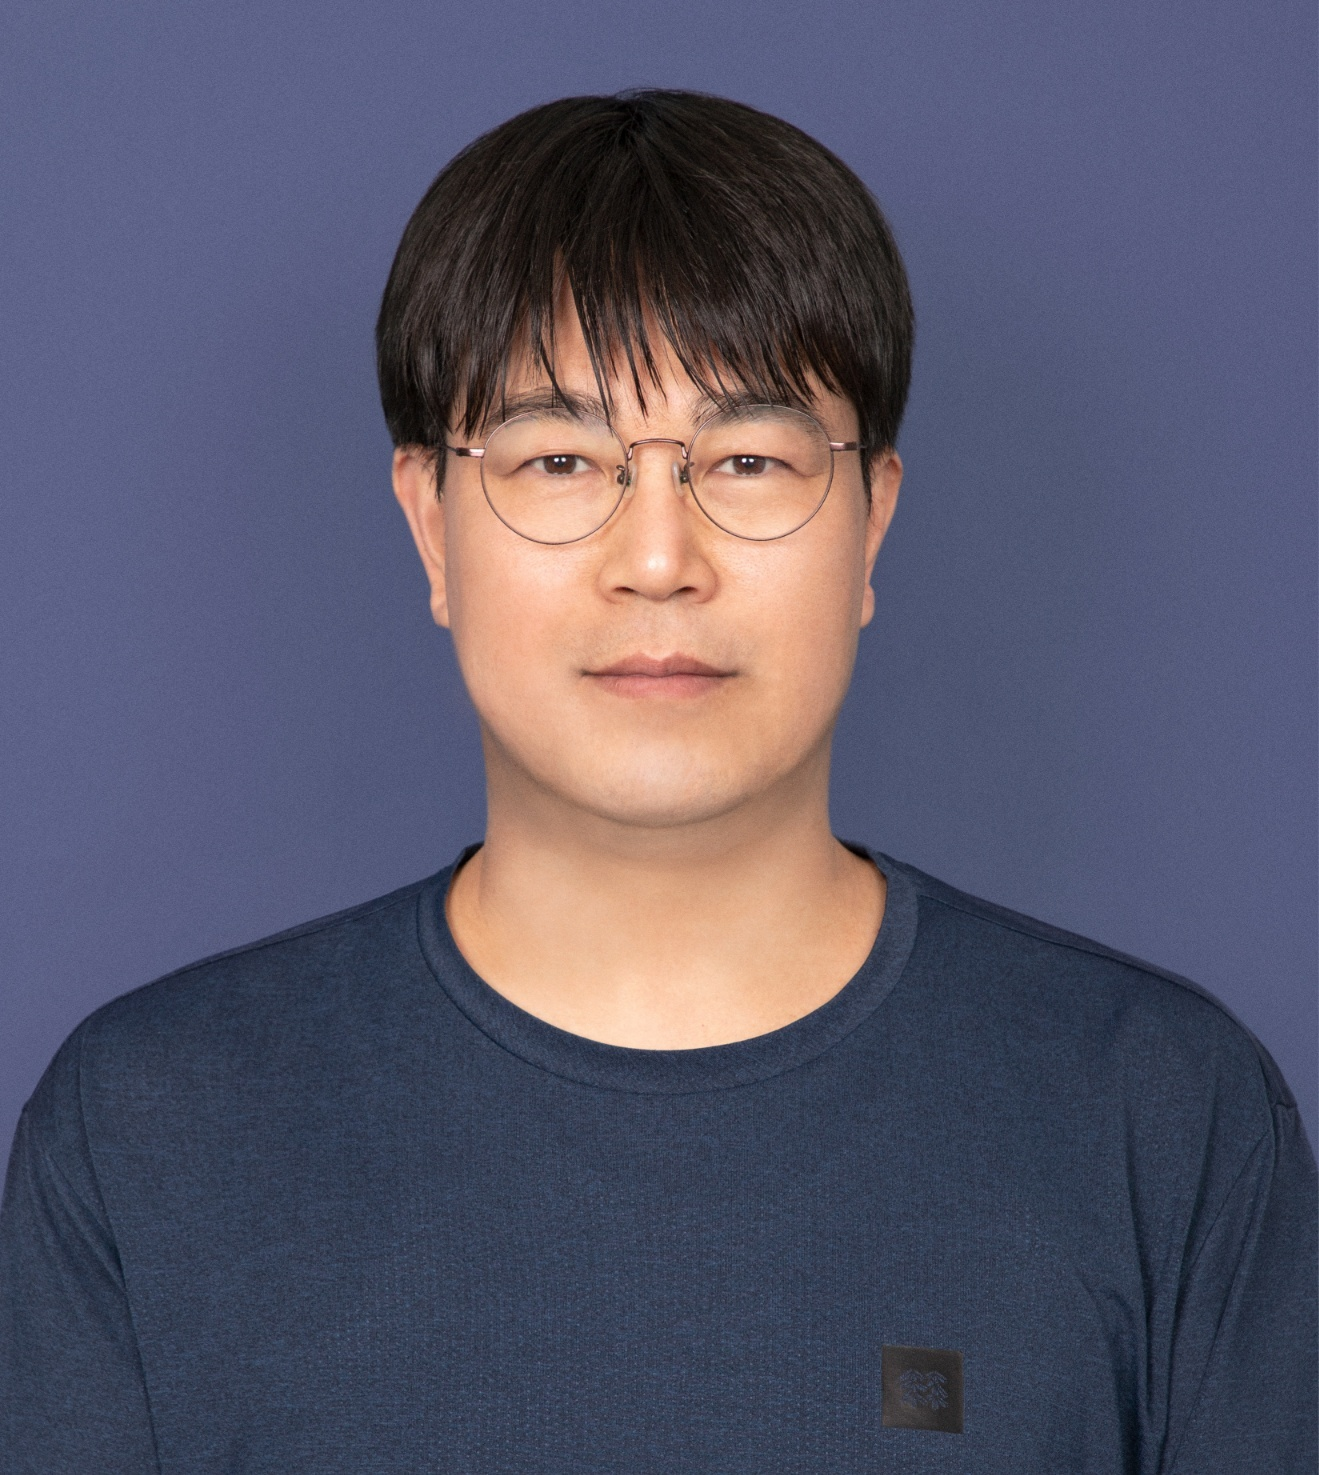
\includegraphics[width=1in,height=1.25in,clip,keepaspectratio]{./fig_author-lim2.png}}]{Geunsik Lim}
received the B.S. degree in Computer Science and Engineering from Ajou University, South Korea, in 2003, and the M.S. and Ph.D. degrees in Electrical and Computer Engineering from Sungkyunkwan University, South Korea, in 2014 and 2023, respectively. He is currently a principal software engineer at Samsung Electronics in South Korea. His research interests include system optimization, operating systems, software platforms, and on-device artificial intelligence. 
\end{IEEEbiography}
\end{minipage}


\end{document}
